%\documentclass[twocolumn,lengthcheck,superscriptaddress]{revtex4-1}

\documentclass[11pt]{amsart}
\usepackage{geometry}                % See geometry.pdf to learn the layout options. There are lots.
\geometry{a4paper}                   % ... or a4paper or a5paper or ... 
%\geometry{landscape}                % Activate for for rotated page geometry
%\usepackage[parfill]{parskip}    % Activate to begin paragraphs with an empty line rather than an indent
\usepackage{color}
\usepackage{graphicx}
\usepackage{amsmath}
\usepackage{amssymb}
\usepackage{amsthm}
\usepackage{epstopdf}
\usepackage{mathrsfs}
\usepackage{enumerate}
\usepackage{xypic}
\usepackage[shortalphabetic]{amsrefs}

\usepackage{hyperref}

\newcommand{\red}[1]{\textcolor{red}{#1}}

\DeclareMathOperator{\supp}{supp}
\DeclareMathOperator{\tr}{tr}
\DeclareMathOperator{\im}{Im}
\DeclareMathOperator{\vspan}{span}
\DeclareMathOperator{\res}{res}

\theoremstyle{plain}% default
\newtheorem{theorem}{Theorem}[section]
\newtheorem{lemma}[theorem]{Lemma}
\newtheorem{proposition}[theorem]{Proposition}
\newtheorem*{corollary}{Corollary}

\theoremstyle{definition}
\newtheorem{definition}{Definition}[section]
\newtheorem{conjecture}{Conjecture}[section]
\newtheorem{example}{Example}[section]

\theoremstyle{remark}
\newtheorem*{remark}{Remark}
\newtheorem*{note}{Note}

%\bibliographystyle{amsalpha}

\title{What is a quantum field state?}
\date{\today}                                           % Activate to display a given date or no date


\begin{document}

\begin{abstract} 
There has been in a fruitful interplay of ideas between quantum information theory and high energy physics, especially in the context of quantum simulation, the AdS/CFT correspondence, and the black hole information loss paradox. However, a core difficulty faced by quantum information theorists -- who are usually concerned with qubits -- interested in these emergent and vibrant areas is the necessity of dealing with quantum fields. The primary purpose of these notes is to lower the entry barrier for quantum information theorists to work on these topics by explaining what, in a quantum information friendly way, a quantum field state actually is. We describe the Wilsonian formulation of quantum field theory as an effective theory and explain how this leads naturally to a definition, independent of lagrangians, of quantum field states which is better adapted to, e.g., tensor networks. We hope that there is something here for high-energy theorists as well, if only to see how someone from ``the other side'' thinks about complex quantum systems.
\end{abstract}

\maketitle

\section{Introduction}
Quantum field theory (QFT) has become, thanks to Wilson 
\cite{wilson_renormalization_1974,wilson_renormalization_1975}, an immensely powerful calculational machine to study a wide variety of physical problems from the fundamental physics of particles \cite{peskin_introduction_1995,weinberg_quantum_1996,weinberg_quantum_1996-1,weinberg_quantum_2000} to many body interacting quantum systems such as magnets and dilute atomic gases \cite{fradkin_field_2013}. It is no exaggeration to say that QFT is the calculus of modern physics \cite{witten_surface_2006,seiberg_nathan_2014}. In contrast to the mature status that calculus enjoys, however, QFT is still far from a stable formulation \cite{howard_georgi_particles_2012,moore_physical_2014,seiberg_nathan_2014} as texts on the subject are not standardised and, further,  mathematicians are not yet universally happy with QFT as practiced by physicists. 

Amongst the many formulations of QFT, a most popular one is in terms of \emph{lagrangians}. Here one begins with a set of \emph{classical} equations of motion, encapsulated by a lagrangian via the principle of least action \cite{arnold_mathematical_1989}, and then seeks a \emph{quantisation} of these equations of motion, typically via the path integral prescription. This approach has led to great progress: for example, it works extremely well in the perturbative setting, where quantum field theory is on firm footing and, more importantly, it also provides an elegant way to approach the \emph{nonperturbative} setting where, e.g., it serves as the basis of lattice gauge theory \cite{creutz_quarks_1985,wilson_confinement_1974}. In the case of lattice gauge theory a dramatic validation of the path integral formulation was recently obtained when the hadronic spectrum of QCD was numerically obtained from first principles \cite{durr_ab_2008}. However, despite the power and ubiquity of the lagrangian/path integral approach, there are still many mysteries concerning nonperturbative QFT.  

One way to make progress on understanding nonperturbative QFT might be to eschew the lagrangian parametrisation altogether. This is not a new idea: in the '60s and '70s the idea of deriving all of physics from the analyticity properties \cite{eden_analytic_2002} of the $S$ matrix was very popular. This idea lost steam\footnote{This is actually not fair: the $S$ matrix bootstrap programme was one of the starting points for string theory, which has subsequently enjoyed tremendous success in understanding QFT, especially via dualities. This is a vast topic which lies beyond the scope of these notes. Here we largely focus on non-string approaches to QFT.} in the late '70s in the wake of the stunning success of the standard model. Recently, however, there has been an upswing in interest in formulations of QFT without the lagrangian. A major impetus here comes from string theory \cite{moore_physical_2014,howard_georgi_particles_2012} where there are arguments that there exist certain quantum field theories \cite{witten_comments_1995,moore_lecture_2012} with no known, or no unique, lagrangian. Additional motivation for studying QFT without lagrangians has been powerfully articulated by Arkani-Hamed and collaborators in the course of a programme to understand the scattering amplitudes for $\mathcal{N}=4$ supersymmetric Yang-Mills theory \cite{arkani-hamed_what_2010,arkani-hamed_into_2014,arkani-hamed_tree_2008,arkani-hamed_scattering_2012,arkani-hamed_all-loop_2011,arkani-hamed_amplituhedron_2014,arkani-hamed_s-matrix_2010,arkani-hamed_what_2010}: here the core motivation is to find a parametrisation of QFT which exposes hidden symmetries at the expense of  manifest unitarity and locality, i.e., to allow spacetime to be an emergent property.  

The theme of emergent spacetime plays a crucial role in discussions of the \emph{holographic principle} \cite{bousso_holographic_2002}. In the specific context of the AdS/CFT correspondence \cite{maldacena_large_1999} we have seen that spacetimes of certain associated bulk degrees of freedom are encoded in the Hilbert spaces of strongly interacting quantum many body systems living on spatial boundaries. The nature of this encoding is still not completely understood, particularly away from the large-$N$ limit where semiclassical arguments are no longer valid. However, this idea has proved to be so deep that even just taking aim in its general direction has lead to spectacular and exciting progress. Most relevant for this paper is a line of enquiry beginning with the work of Swingle \cite{swingle_entanglement_2012} applying tensor networks to quantify the nature of, and the correspondence between, bulk and boundary degrees of freedom \cite{nozaki_holographic_2012,ryu_aspects_2006,ryu_holographic_2006}. Also closely related, are studies exploiting quantum information theoretic ideas, particularly from the study of quantum error correcting codes \cite{almheiri_bulk_2014,pastawski_holographic_2015} and quantum Shannon theory \cite{czech_information_2014}, aimed at elucidating the interpretation of AdS/CFT duality. These recent studies usually work by first discretisating the problem and then deploying the apparatus of quantum information theory to the resulting discrete system. The precise way in which results obtained in this way survive the limit to the continuum is rather subtle.

Continuing with the themes of holography, emergent spacetime geometry, and quantum information theory, there has been a recent flurry of activity centred around the ``firewall'' paradox, initiated by the work of \cite{almheiri_black_2013}. The ensuing debate has prompted many intriguing and original ideas aimed at resolving the paradox. One extremely suggestive proposal \cite{maldacena_cool_2013}, known as ``ER=EPR'', posits that the fabric of spacetime itself is none other than quantum entanglement. This is heady stuff! However it is hard, especially for the quantum information theorist, to make concrete sense of it, especially since at first sight the proposal appears to be a category error. 

We believe that quantum information theorists have interesting things to contribute to high energy physics, and see several possible avenues forward. The most direct way would be to develop ideas and results that have already proved successful in the study of strongly correlated complex quantum systems to apply to settings of direct interest in high energy physics. In this context, new variational families of \emph{tensor network states} (TNS), including, the \emph{projected entangled pair states} (PEPS) \cite{verstraete_renormalization_2004} and the \emph{multiscale entanglement renormalisation ansatz} (MERA) \cite{vidal_entanglement_2007,vidal_class_2008} could be exploited. The crucial idea underlying these developments is that TNS provide a parsimonious and expressive \emph{data structure} to parametrise  the Hilbert space of physical states naturally arising \cite{poulin_quantum_2011} in local quantum systems \cite{orus_practical_2014, haegeman_geometry_2014,osborne_simulating_2007,bravyi_topological_2010,bravyi_short_2011,hastings_lieb-schultz-mattis_2004,hastings_area_2007,osborne_efficient_2006}. One way to carry out the goal of understanding quantum fields via tensor network methods is to formulate TNS directly in the continuum. This approach has already given rise to the continuous matrix products states (cMPS) \cite{verstraete_continuous_2010,osborne_holographic_2010, haegeman_calculus_2013}, continuous PEPS \cite{jennings_variational_2012}, and continuous MERA classes \cite{haegeman_entanglement_2013}. Such continuous TNS have provided some new insights in the study of some problems in high-energy physics, and promise to provide a powerful way to reason about entangled quantum fields. Another way, adopted in this paper, is to simply understand how discrete TNS approximate a given QFT. This approach is easier to implement numerically, and also more directly allows the computation of, e.g., quantum entanglement.

Another avenue where quantum information theory seems likely to lead to progress in high energy physics is by exploiting quantum computers to directly simulate scattering processes. This is an important goal, even in the perturbative setting, because quantum computers allow the computation of scattering amplitudes involving many particles requiring the summation of a prohibitive number of Feynman diagrams. Pursuit of this idea has led to the development of discrete quantum simulation algorithms for scalar field theory \cite{jordan_quantum_2012,jordan_quantum_2011} and the Gross-Neveu model on the lattice \cite{jordan_quantum_2014}. Here there are again fascinating questions about how to understand the nonperturbative regime and the approach to the continuum.  

Finally, and somewhat more speculatively, the work \cite{arkani-hamed_what_2010,arkani-hamed_into_2014,arkani-hamed_tree_2008,arkani-hamed_scattering_2012,arkani-hamed_all-loop_2011,arkani-hamed_amplituhedron_2014,arkani-hamed_s-matrix_2010,arkani-hamed_what_2010} of Arkani-Hamed and collaborators is rather suggestive to someone with a quantum information background: the idea that scattering amplitudes can be directly obtained from the volumes of a certain special convex set known as the \emph{amplituhedron} resonates strongly with themes that have been discussed in the quantum information literature. In particular, the amplituhedron bears a superficial resemblence to the convex set of reduced density operators for (translation invariant) complex quantum systems \cite{verstraete_matrix_2006,zauner_symmetry_2014}. For instance, one can argue that scattering amplitudes for any complex quantum system may be directly derived from knowledge of a related convex set \cite{osborne_tobiasosborne}. Whether the connection between these two topics is more than metaphoric is far from clear, however, it seems like a deep idea worth exploring further. 

So it seems that there are a variety of ways in which quantum information theory could contribute to high energy theory. However, there is a fundamental difficulty facing the quantum information theorist:  quantum fields involve a continuous infinity of degrees of freedom, a setting rather far removed from the home ground of quantum information theory, namely, the qubit. Faced with the insecurity of exploring such unfamiliar territory it is tempting to work from a comfortable rigourous mathematical formulation. However,  a satisfying universally accepted mathematical framework for QFT has yet to be found; there are a panoply of existing approaches from the algebraic, probabilistic, to the geometric (we are lucky in that we can simply refer to an excellent recent survey of Douglas \cite{douglas_foundations_2012}, who provides a broad overview of the existing approaches to a mathematical theory of QFT). It is certainly possible that quantum information theory could contribute to high energy physics via one of the aforementioned mathematical approaches. However, we now end up with two problems, namely, understanding and developing quantum information ideas for a given mathematical approach, and then working out how to apply them to physical problems. 

The approach adopted in these notes is rather different. Here we advocate directly understanding QFT as practiced by physicists. This differs in two important ways from most of the existing mathematical approaches that have been so far developed. Firstly, we regard QFT as an \emph{effective theory} and, secondly, we focus on quantum \emph{state space} in addition to quantum observables. By understanding the way QFT is formulated as an effective theory, we can avoid a lot of heavy mathematical machinery and get down to concrete problems and calculations. 

So what is a quantum field state? Our answer is that it is a \emph{sequence of states} of discretised theories with a certain property, namely, that each term gets closer to each other (i.e., a \emph{Cauchy sequence}). This is directly analogous to how we study, via computer, classical fields, like fluids and gases and the electromagnetic field. Following in the footsteps of Wilson, we spend some time discussing how to measure ``closeness'', leading to the introduction of a family of quantum information distance measures quantifying the large-scale behaviour of a quantum many body state. 

We've structured this paper as follows. We begin in \S\ref{sec:opqp} with a short overview of operational quantum mechanics with an emphasis on density operators, completely positive maps, and POVMs. After setting up this basic language we move on in \S\ref{sec:quant} to a short overview of the problems of quantisation. Then we discuss in \S\ref{sec:whatisqft}, on a purely heuristic level, what a field theory really ought to be. With this motivation in hand we then discuss effective theories in \S\ref{sec:effectivetheories}, which directly leads to the Wilsonian formulation of effective quantum field theory, reviewed in \S\ref{sec:wilson}. This discussion is then used as the direct motivation for our definition of effective quantum field states in \S\ref{sec:effectiveqftstates}. The construction of quantum field states via completion is then introduced in \S\ref{sec:qftcompletion}. The explanation of the renormalisation group as a means to construct Cauchy sequences of states is then described in \S\ref{sec:cauchyseqrg}. Finally, we conclude with some discussion and outlook in \S\ref{sec:discussion}.

A final note: in preparing these notes we had in mind a list of questions that any putatitive field theory formulation should answer. This list includes
\begin{enumerate}
	\item What is a continuum limit actually, and how do we compare between the continuum and the discretuum?
	\item ...
\end{enumerate}

\section{Operational quantum physics}\label{sec:opqp}
Throughout these notes we emphasise the \emph{operational} or \emph{modular}\footnote{Modular refers, in this context, to the idea that the primitive operations of preparation, evolution, and measurement may be composed arbitrarily to build \emph{quantum circuits}, much as we do in building classical circuits.} \emph{viewpoint}: here the focus is on physical quantities with an \emph{operational interpretation}, i.e., a physical quantity is considered operationally meaningful only if there exists, at least in principle, an experiment which could measure it. The modular viewpoint is common within the quantum information community as it lends itself very naturally to the discussion of quantum circuits. The operational view also seems to mesh rather well with the Wilsonian view of QFT, where QFT is seen as an effective theory.

A convenient way to discuss quantum physics within the operational or modular viewpoint is via \emph{observables and effects}, \emph{density operators}, and \emph{completely positive maps} \cite{ludwig_foundations_1983,davies_quantum_1976}. This language may be unfamiliar to the reader and we pause a moment to review it here. Firstly, the way we characterise \emph{quantum} (indeed, also \emph{classical}) systems is via a set $\mathcal{A}$ of \emph{observables}. The observables typically form an algebra isomorphic to the bounded operators $\mathcal{B}(\mathcal{H})$ on some Hilbert space $\mathcal{H}$, although this is not necessary\footnote{The algebra structure is usually employed as a proxy for \emph{positivity}. All that we actually need is that $\mathcal{A}$ is an \emph{Archmidean Order Unit} (AOU) vector space \cite{paulsen_vector_2009,kleinmann_typical_2013}.} for there to be a probability interpretation. For the probability interpretation we need only require that $\mathcal{A}$ has a notion of \emph{positivity}, i.e., there is a cone $\mathcal{A}^+ \subset \mathcal{A}$ of positive elements and that there is a distinguished unit element $\mathbb{I}\in\mathcal{A}$ which is also positive. A good example to keep in mind here is that of the \emph{qubit}, where $\mathcal{A}\equiv M_2(\mathbb{C})$, the algebra of $2\times 2$ complex matrices and $\mathcal{A}^+ \equiv \{M\in \mathcal{A}\,|\, M\ge 0\}$ (with $\ge$ denoting the positive semidefinite order, i.e., $M\ge 0$ if and only if there exists $A\in \mathcal{A}$ such that $M = A^\dag A$). Another example is that of a \emph{classical} system, which is characterised by a \emph{commutative algebra} $\mathcal{A}\equiv \mathcal{C}(X)$, the set of functions from some set $X$ to $\mathbb{C}$; a \emph{classical bit} corresponds to the choice $X \equiv \{0,1\}$. An \emph{effect} $E\in\mathcal{A}^+$ is then what we call an observable corresponding to an \emph{outcome}, \emph{proposition}, \emph{predicate}, or \emph{yes/no measurement}. It is characterised by the property that $0\le E\le \mathbb{I}$. The unit element is the effect corresponding to the empty predicate, that is, no assertion. For the qubit example above the projector $P_0 = \left(\begin{smallmatrix} 1 & 0 \\ 0 & 0\end{smallmatrix}\right)$ is the effect corresponding to the assertion that the system is in the ``zero'' configuration. A POVM\footnote{The acronym POVM stands for ``positive operator valued measure'', which takes its full meaning when the observable can take a continuous sets of values. } corresponds to a measurement of a system and---provided it can take only finitely many values---comprises of a set $\mathcal{M} = \{E_j\}_{j=1}^n$ of effects such that 
\begin{equation}
	\sum_{j=1}^n E_j = \mathbb{I}.
\end{equation}
The subscript label $j$ is what carries the information about what \emph{outcome} was observed when the measurement took place. It can be interpreted directly as the \emph{value} of the observable being measured, or simply as a label of that value. It is worth stressing that the effects $E_j$ need not be projections. Traditionally we speak of hermitian operators as observables in quantum mechanics, but what is actually meant when we declare that the hermitian operator $M = \sum_{j=1}^n m_j E_j$ is an ``observable'' is that we implement the corresponding POVM  $\mathcal{M} = \{E_j\}_{j=1}^n$, where $E_j$ are the spectral projections for $M$. The expectation value $\langle M \rangle$ corresponds to the first moment of the probability distribution determined by $\mathcal{M}$.

Quantum composition of systems is described via the \emph{tensor product} operation: suppose we have two systems $A$ and $B$ characterised by the observable sets $\mathcal{A}_A$ and $\mathcal{A}_B$, respectively. The joint system $AB$ is then characterised by the observable set $\mathcal{A}_{AB} \equiv \mathcal{A}_A\otimes \mathcal{A}_B$. This space allows the simultaneous observation of effects in both $\mathcal{A}_A$ \emph{and} $\mathcal{A}_B$. The \emph{classical composition} of two systems $\mathcal{A}_A$ and $\mathcal{A}_B$, where we allow the observations of effects in \emph{either}  $\mathcal{A}_A$ \emph{or} $\mathcal{A}_B$, i.e., our system is either of one type or another, is described by the \emph{direct sum} operation $\mathcal{A}_{A}\oplus \mathcal{A}_B$. This is the smallest space of effects allowing us to probabilistically measure an effect from  $\mathcal{A}_A$ or $\mathcal{A}_B$.

A \emph{state} $\omega:\mathcal{A}\rightarrow \mathbb{C}$ on the observable set $\mathcal{A}$ is a \emph{positive}, \emph{normalised}, and \emph{linear} functional, i.e., $\omega:\mathcal{A}^+\rightarrow \mathbb{R}^+$ and $\omega(e) = 1$. A state describes a \emph{preparation} of the system, and captures all the information relevant for the statistical outcomes of measurements on the system. The probability $p_E$ that, after a measurement of a POVM $\mathcal{M}$, an outcome with corresponding effect $E$ occurs is given by $p_E = \omega(E)$. Usually in quantum information theory we work with finite-dimensional quantum systems with $\mathcal{A}\equiv M_d(\mathbb{C})$ so that we can represent states via \emph{density operators} $\rho\in M_d(\mathbb{C})$ according to $\omega(M) \equiv \tr(\rho M)$, with $\tr(\rho) = 1$, $\rho \ge 0$. (Be aware that in infinite-dimensional settings it is not always possible to find a density operator corresponding to a state as the trace condition can easily fail.) A state $\omega$ is \emph{pure} if it cannot be written as a convex combination of other states, i.e., if $\omega \not= p \omega' + (1-p) \omega''$, with $p\in (0,1)$. Continuing the qubit example from above we see that single-qubit states $\omega$ correspond to $2\times 2$ density operators 
\begin{equation}
	\rho = \frac{\mathbb{I} + \mathbf{r}\cdot \boldsymbol{\sigma}}{2},  
\end{equation}  
with $\boldsymbol{\sigma} \equiv \left[\left(\begin{smallmatrix} 0 & 1 \\ 1 & 0\end{smallmatrix}\right), \left(\begin{smallmatrix} 0 & -i \\ i & 0\end{smallmatrix}\right), \left(\begin{smallmatrix} 1 & 0 \\ 0 & -1\end{smallmatrix}\right)\right]$. We have that $\omega(\sigma^j) = \tr(\rho \sigma^j)$. The condition that $\rho$ corresponds to a state translates to the condition that $|\mathbf{r}| \le 1$. Pure qubit states are precisely those with $|\mathbf{r}| = 1$.

The most general dynamical process that can occur within quantum mechanics is represented by a \emph{completely positive map} (CP map), or \emph{channel}. These processes describe everything from preparations, time evolutions, measurements, to the addition of ancilla and the discarding of subsystems. The input and output of a CP map may be arbitrary: there is no especial difficulty in the formulation caused by, e.g., different numbers of input and output systems. We first describe CP maps in the \emph{heisenberg picture} where modifications of measurements are specified. Here a CP map $\mathcal{E}$ is characterised by the following three axioms: 
\begin{enumerate}
	\item it is a \emph{linear} map $\mathcal{E}:\mathcal{A}_B\rightarrow \mathcal{A}_A$ from the observables $\mathcal{A}_B$ of an \emph{output system} $B$ to the observables of $\mathcal{A}_A$ of the  \emph{input system} $A$;
	\item the map $\mathcal{E}$ is \emph{positive}, i.e., it takes positive elements to positive elements according to $\mathcal{E}:\mathcal{A}_B^+\rightarrow \mathcal{A}_A^+$; and 
	\item running the map $\mathcal{E}$ in parallel with the \emph{identity channel} $\mathcal{I}_E : \mathcal{A}_E\rightarrow \mathcal{A}_E$ on an arbitrary auxiliary system $\mathcal{A}_E$ yields a positive linear map $\mathcal{E}\otimes \mathcal{I}_E$ from $\mathcal{A}_B\otimes \mathcal{A}_E$ to $\mathcal{A}_A\otimes \mathcal{A}_E$.
\end{enumerate} 
Pleasingly this axiomatic characterisation of a general dynamical process matches the following constructive characterisation. Suppose we only allow maps which comprise of the following three primitives: (1) adjunction of  ancillary systems; (2) unitary transformations; and (3) reduction to a subsystem. Then it is a result of Stinespring that such operations correspond precisely to CP maps and vice versa. 
\begin{theorem}[Stinespring] Suppose that $\mathcal{A}_A \equiv M_m(\mathbb{C})$ and $\mathcal{A}_B \equiv M_n(\mathbb{C})$. Then a linear map $\mathcal{E}:\mathcal{A}_B\rightarrow \mathcal{A}_A$ is completely positive if an only if there is an auxiliary system $\mathcal{A}_E \equiv M_l(\mathbb{C})$ such that it takes the form
\begin{equation}
	\mathcal{E}(X) = V^\dag (X\otimes \mathbb{I}_E) V,
\end{equation}
where $V$ is an operator from $\mathbb{C}^m$ to $\mathbb{C}^n\otimes\mathbb{C}^l$. Further, $V$ is an isometry whenever $\mathcal{E}$ is \emph{unital}, i.e., $\mathcal{E}(\mathbb{I}) = \mathbb{I}$. 
\end{theorem}
Here $V$ describes both the unitary dynamics and the reduction to a subsystem and $X\mapsto X\otimes \mathbb{I}$ describes the adjunction of the ancillary system. 

There are several key examples of CP maps naturally arising in physics.  The first examples are the so-called \emph{cq channels} (cq = classical-quantum), describing \emph{preparations}: these are channels from a set of quantum observables $\mathcal{A}$ to classical observables $\mathcal{C}(X)$ with $X \equiv \{1,2,\ldots, n\}$,
\begin{equation}
	\mathcal{E}(E) \equiv \sum_{j = 1}^n \omega_j (E) \delta_j,
\end{equation}
where $\{\omega_j\}_1^{n}$ are a set of states on $\mathcal{A}$, and $\delta_j$ is the delta function on $\{1,2,\ldots, n\}$, i.e., $\delta_j(k) = \delta_{jk}$. 

The second important subclass of channels are those describing \emph{evolutions} according to \emph{unitary dynamics}: these CP maps are nothing more that conjugation by a unitary operator $U$
\begin{equation}
	\mathcal{U}(X) \equiv U^\dag X U.
\end{equation}

The final essential example of a channel is the \emph{qc channel} describing a POVM measurement
\begin{equation}
	\mathcal{M}(\delta_j) \equiv E_j.
\end{equation}

Using channels we can expose the modular structure of general processes in quantum mechanics, where components can be combined and concatenated: we draw classical information with a double line and quantum states with a single line. The passage of time is thought of as flowing from left to right. Channels are represented as boxes with input and output lines. Accordingly, any experiment in physics ultimately corresponds to the combination of a preparation, an evolution, and a measurement. We represent this pictorially represented as follows.
\begin{center}
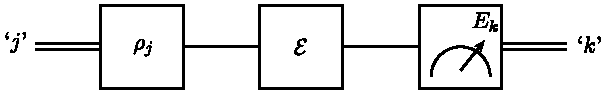
\includegraphics{prepevolvemeasure.pdf}
\end{center}
Here, conditioned on a classical input with the value $j$, a quantum state $\rho_j$ is prepared. This is subsequently evolved according to a completely positive map $\mathcal{E}$. Finally a POVM measurement $\mathcal{M} = \{E_k\}$ is performed producing the classical output $k$. Although this modular view of quantum mechanics won't be directly exploited in the sequel, it is present in our minds when we come to discussing the building blocks of quantum field theory. 


Thus, from now on, when we say the word ``theory'' we take this to mean the specification of a triple $(\mathcal{A}, \mathcal{E}_t, \omega)$ of an observable set $\mathcal{A}$, a family of CP maps $\mathcal{E}_t: \mathbb{R}\times\mathcal{A}\rightarrow \mathcal{A}$ of possible evolutions, and a preparation $\omega$. We think of $\mathcal{A}$ as the space of \emph{equal-time} observables. The channel $\mathcal{E}_t$ is what implements the operation of translation in \emph{time}\footnote{In the case where the theory admits an action of a larger group $G$ of, say, spacetime translations, or Poincar\'e transformations, we then suppose that $\mathcal{E}_g$ is indexed by elements of $g\in G$.}. It is convenient to exploit the shorthand notation $A(t) \equiv \mathcal{E}_t(A)$. Thus we can now discuss observables corresponding to measurements at different times. In the case where $\mathcal{A}$ has an algebraic structure\footnote{In the case where $\mathcal{A}$ does not have an algebraic structure we have to explicitly describe correlation functions via instruments.} this allows us to introduce the observables corresponding to $n$-point correlation functions, namely, 
\begin{equation}
	A_1^\dag(t_1)A_2^\dag(t_2)\cdots A_n^\dag(t_n)A_n(t_n) \cdots A_2(t_2)A_1(t_1),
\end{equation} 
where $A_j(t_j) \in \mathcal{A}$, $j= 1,2, \ldots, n$. If $\omega$ is a state represented with density operator $\rho$ on $\mathcal{A}$ the resulting correlator is
\begin{multline}
	\langle A_1^\dag(t_1)A_2^\dag(t_2)\cdots A_n^\dag(t_n)A_n(t_n) \cdots A_2(t_2)A_1(t_1) \rangle =\\ \tr( A_n(t_n) \cdots A_2(t_2)A_1(t_1)\rho A_1^\dag(t_1) A_2^\dag(t_2) \cdots A_n^\dag(t_n)).
\end{multline}
This correlator may be implemented via postselection on the instrument carrying out the measurement of $A_j(t_j)$. 
Note that a ``standard'' $n$-point correlation function $\langle A_n(t_n) \cdots A_2(t_2)A_1(t_1) \rangle$ is not directly measurable in quantum mechanics as, in general, the product $A_n(t_n) \cdots A_2(t_2)A_1(t_1)$ is not even hermitian. Instead, such correlators must be inferred from scattering \cite{taylor_scattering_2006} or interference experiments \cite{glauber_quantum_1963,mandel_optical_1995}.

\section{Quantisation isn't a mystery, it's an inverse problem}\label{sec:quant}
Before we get started with quantum field states we pause a moment to stress a simple yet important point: the universe didn't become quantum in 1927 at the Fifth Solvay International Conference, it has always been quantum. The reason that we didn't notice quantum effects for such a long time is because of \emph{decoherence} \cite{joos_decoherence_2003,gardiner_quantum_2010}, i.e., the unavoidable loss of quantum coherence due to uncontrolled interactions with unobservable environment degrees of freedom. In the presence of quantum noise pure unitary dynamics described by a unitary channel $\mathcal{U}_t$ obeying 
\begin{equation}
	\frac{d}{dt}\mathcal{U}_t(X) \equiv -i [H, \mathcal{U}_t(X)]
\end{equation}
is modified \cite{davies_quantum_1976} to a noisy CP map $\mathcal{E}_t$ generated by 
\begin{equation}
	\frac{d}{dt}\mathcal{E}_t(X) \equiv -i [H, \mathcal{E}_t(X)] -\frac12\sum_{\alpha=1}^m L_\alpha^\dag L_\alpha \mathcal{E}_t(X) + \mathcal{E}_t(X) L_\alpha^\dag L_\alpha - 2 L_\alpha \mathcal{E}_t(X) L_\alpha^\dag
\end{equation}
which can, for quantum systems with a continuous degree of freedom (e.g., a particle on the line), usually be \emph{very effectively} modelled by a symplectic transformation on a classical phase space. 
\begin{center}
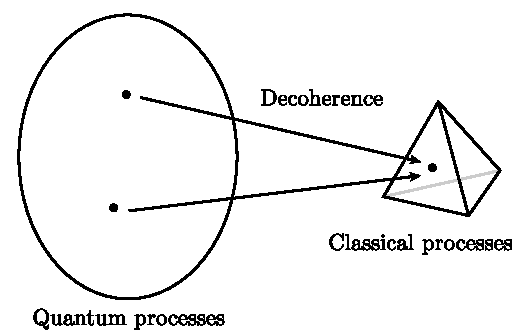
\includegraphics{Decoherence.pdf}
\end{center}
The map, induced by decoherence, between a unitary quantum process and an effective classical process is extremely nonlinear and complicated. However, the most relevant feature of decoherence for this discussion is simply that many different quantum dynamical processes can be, after decoherence has set in, effectively modelled by the \emph{same} classical dynamical system. Thus the decoherence map is, amongst other things, a \emph{many to one} map. Thus, when presented with a given classical dynamical system we have no way, not even in principle, of identifying the ``correct'' quantisation; we are trying to invert a many to one map and there is no canonical choice of preimage.  None of this is really surprising or controversial. (Note that the \emph{semiclassical limit} is \emph{not} the same as the \emph{effective classical limit} arising from the presence of decoherence. While there is, in both cases, an emergence of classicality from a quantum system, the reasoning is totally different.)

Quantisation is hard precisely because we are trying to simultaneously solve more than one problem at once: we are trying to find a quantum system such that when we solve the system in the presence of decoherence, we find it is well described by a classical effective theory which matches the originally specified classical system. Said this way it is truly a miracle that the bewildering variety of quantisation recipes developed over the past decades work at all! 
\begin{center}
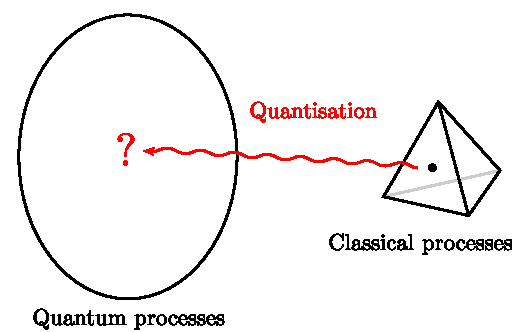
\includegraphics{Quantisation.pdf}
\end{center}
From this perspective it isn't so surprising that quantisation prescriptions aren't universal maps between classical systems and quantum systems, i.e., in mathematical language, \emph{functors}. 

So how is the inverse problem of quantisation solved? A vitally important role guiding us toward a solution is played by \emph{symmetries}: if a desired classical limit is invariant under some group of symmetry operations then it is reasonable to assume that a good quantisation ought to furnish some representation of the same symmetry group (especially if the envisaged decoherence process leading to the classical limit is not expected to break the symmetry). This radically cuts down the search space we need to cover in looking for a quantisation. It can turn out, however, that the full symmetry group cannot be represented in a given quantisation, in which case we say that one or more symmetries are \emph{anomolous}. It is an interesting question whether, in general, anomolies disappear in the classical limit under a reasonable model of decoherence.

In the more modular language promoted in these notes we simply simplistically regard decoherence as a channel $\mathcal{D}$ that gets applied to our system before we perform our measurements. Thus, in the heisenberg picture, you can think of decoherence as modifying the effects we can measure to more noisy effects.  

\section{What is a field theory}\label{sec:whatisqft}
We begin our discussion by contemplating, at a purely heuristic level, what a \emph{field theory} should be. On a purely intuitive level, a \emph{field} (either quantum or classical) comprises \emph{continuously} many degrees of freedom, i.e., roughly speaking, there is a degree of freedom for each point in space $\mathbb{R}^d$ (or spacetime $\mathbb{R}\times \mathbb{R}^d$). When dealing with such a vast abundance of degrees of freedom the task of just specifying a state of such a field becomes deeply nontrivial. 

Classically, this task is largely solved by calculus. Here \emph{pure field states} can be simply defined to be continuous functions $\phi:\mathbb{R}^d\rightarrow \mathbb{R}$. The space $C(\mathbb{R}^D)$ (or, in the case of spacetime, $C(\mathbb{R}\times\mathbb{R}^D)$) of all \emph{mathematically} possible such field states is rather wild -- it contains fractal monsters -- but not all of the states in $C(\mathbb{R}^D)$ are meant to be \emph{physically realisable}. Classically we specify physical pure states by requiring that they satisfy certain differential equations. For example, in a $(1+1)$-dimensional spacetime of points $(t,x)\in \mathbb{R}^2$ we could demand that valid physical states satisfy
\begin{equation}
	\frac{\partial^2\phi}{\partial t^2} - \frac{\partial^2\phi}{\partial x^2} + m^2\phi = 0.
\end{equation}
Just to be a solution of such an equation of motion implicitly requires that $\phi$ is at least twice differentiable. (Leaving aside, for the moment, the topic of weak solutions and distributions.) The condition of differentiability is actually rather nontrivial as it means that at small scales any solution is quite boring (it is basically a straight line) when we zoom in:
\begin{center}
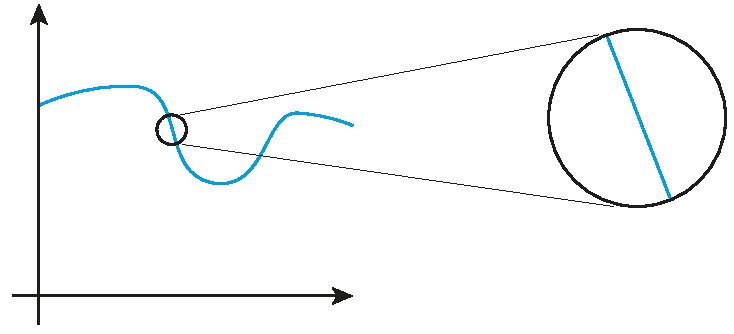
\includegraphics{difffunc.pdf}
\end{center}
While this doesn't help us solve the problem of building statistical theories of classical fields -- the task of understanding probability measures on infinite dimensional spaces is deeply nontrivial -- it does at least allow us to tame the problem of understanding pure states and their dynamics for systems of continuously many classical degrees of freedom.

But what about quantum theories? Here we encounter a fundamentally new problem not present in the classical case: it is now hard to even define \emph{pure} field states. Naively this should be straightforward: just define the space of pure states to be the tensor product
\begin{equation}
	\mathcal{H}\, \text{``$=$''} \bigotimes_{x\in \mathbb{R}^d} \mathcal{H}_x,
\end{equation}
where $\mathcal{H}_x$ is the Hilbert space for a single degree of freedom located at $x$. The scare quotes here are intended to indicate that the object on the right hand side does not \emph{naively} exist in any satisfying mathematical way\footnote{It does exist in a less naive way via von Neumann's incomplete tensor product. The incomplete tensor product admits an attractive physical intepretation: it is the separable Hilbert space describing the configurations of at most a finite number of particles above the vacuum state. Finite can mean, e.g., $10^{34}$. This doesn't help us, however, as it just pushes our difficulties into building the vacuum.}. But let us be bold physicists for a moment and simply pretend that mathematicians will sort it all out and the space does exist. In this case we ought to have a basis of pure states labelled, e.g., by continuous functions
\begin{equation}
	\{|\phi\rangle \}_{\phi:\mathbb{R}^d\rightarrow \mathbb{R}}.
\end{equation}
While this initially looks reasonable we quickly find a new problem: what superpositions are we going to allow? All of them? Surely not: we must find equations that specify for us the physically realisable states. Here we can no longer take recourse to calculus for help. Indeed, the problem of specifying physically realisable pure states of quantum fields is intimately tied to the problem of writing probability measures for classical fields in one lower spatial dimension via the so called ``classical-quantum'' correspondence where the path integral for a system in $D$ spatial dimensions can be regarded, via Wick rotation, as defining a statistical mechanical system in $D+1$ euclidean dimensions.

In both the classical statistical field and the quantum field cases we have come up against a fundamental physical problem (as opposed to a technical mathematical problem), namely that of specifying interesting states of fields (in the former case, as probability measures, and in the latter as pure states). What we ideally want is a physical principle that tells what are the ``good'', or \emph{physical}, field states versus the ``bad'', or \emph{unphysical}, states.  

\section{Effective field theories}\label{sec:effectivetheories}

Suppose we have some extraordinarily complicated system of many particles -- a good example to keep in mind is \emph{water}. Now if it were easy, \emph{at no cost}, for us to make any conceivable measurement on the system allowed by quantum mechanics, then there is \emph{no way} we'd be fooled into thinking water is anything other than a collection of a vast number of fundamental particles, quarks, gluons, etc., in some incredibly complicated evolving entangled state. The reason we don't see water like this is that we \emph{can't} make any measurement of the system without paying some kind of bill: the more complicated the measurement, the more we have to pay. Thus we have to settle with making measurements of simpler quantities. For example, our eyes are basically a pair of pretty crappy photon detectors and thus when we look at a water sample we are simply carrying out a very noisy and inefficient POVM. Now here is the main point: when you only have access to fewer observables then you can formulate a \emph{simpler hypothesis} which can still explain all the observational data you can obtain. This simpler hypothesis is an \emph{effective theory} for the system. Simpler here can mean many things, but in the context of this paper it is via a field theory\footnote{Why are fields simple? The answer is calculus: it is often easier to calculate integrals than sums.}.

How can we model the large-scale degrees of freedom that we humans with our limited resources can access? One very simplified way is by developing a \emph{zooming out} operation. Since zooming out corresponds to \emph{ignoring information}, this operation should be representable in quantum mechanics as an irreversible CP map $\mathcal{E}$. The reason that it has to be irreversible is that it must prevent us from measuring degrees of freedom that we would otherwise be able to measure: after all, if we could measure all the observables after zooming out that we could measure before then in what sense can we be have said to have zoomed out? In the context of lattice systems there is a very convenient way to implement the zoom-out operation, namely, via Kadanoff blocking. This is the CP map whereby a block of spins is mapped to single spin via the partial trace channel, and then the lattice is rescaled.

Suppose we have some tremendously complicated microscopic system of degrees of freedom at some fundamental length scale $\Lambda$ in some state $\rho_\Lambda$. However, we can only perform limited measurements at our terrestrial length scale $\sigma$ modelled by effects of the form $\mathcal{E}_{\sigma}(E)$, where $E \in \mathcal{A}_{\sigma}$ is an effect in the space of \emph{our} observables. Since we can only measure a handful of all the possible observables $\mathcal{A}_\Lambda$ on the microscopic theory, we are satisfied with the explanation provided by any \emph{effective state} $\rho_{\text{eff}}$ which looks indistinguishable from $\rho_\Lambda$ according to any measurement $\mathcal{E}_{\sigma}(E)$, i.e.\ any state obeying
\begin{equation}
	\tr(\mathcal{E}_{\sigma}(E) (\rho_\Lambda - \rho_{\text{eff}})) \approx 0, \quad \text{for all } E\in \mathcal{A}_\sigma.
\end{equation}
The fewer the observables we can measure, the simpler our hypothesis for $\rho_{\text{eff}}$ can be. In the case of fields, we are only able to measure a handful of observables $E(x)$ indexed by some continuous label $x$; we'll explain this a bit more concretely in the following sections.

One aspect of this discussion may be puzzling for readers familiar with quantum field theories: why are we insisting on saying a change of scale is a lossy operation when, e.g., in CFTs a scale change is a \emph{reversible unitary operation}? The answer is that, in terms of a \emph{microscopic theory} with a cutoff, zooming out \emph{must} be a lossy operation as we can push degrees of freedom past the cutoff. However, in terms of an effective theory, a scale change can be unitary because there is an effective decoupling of the large-scale  and the small-scale degrees of freedom and the action of a finite scale change doesn't, \emph{in the large cutoff limit}, couple the different sets of degrees of freedom. 

A quantum information theorist may find the analogy with noiseless subsystems helpful: if you like, effective theories are analogous to (approximate) decoherence-free subspaces/subsystem codes, where the errors in this case are induced by scale changes. This is a quantitative way to understand what is meant by IR/UV decoupling. If zooming out is a CP map $\mathcal{E}$ then what is ``zooming in'', or \emph{UV completion}? The answer is that there is no unique answer: any CP map $\mathcal{D}$ such that $\mathcal{D}\circ \mathcal{E} \equiv \mathcal{I}$ can be given the interpretation as a zooming in map. That is, first adding details (zooming in) and then removing them (zooming out) should have no effect (recall that we write the channels in the Heisenberg picture, so the order is inverted). Exploiting once more the analogy with noiseless subsystems you can think of zooming in as an error recovery operation $\mathcal{D}$ on the large-scale degrees of freedom. We will return to this point later.

\section{The Wilsonian formulation of effective quantum field theory}\label{sec:wilson}
Here we review, broadly following the expositions of \cite{wilson_renormalization_1975,wilson_renormalization_1974}, \cite{peskin_introduction_1995}, and \cite{moore_lecture_2012}, the Wilsonian view of quantum field theory as an effective field theory. It is \emph{not at all} necessary to understand the discussion here at anything other than a metaphoric level as we are going to revisit the ideas of this section in the sequel to make the intuitive discussions here more concrete. Just read through the description and try and absorb the general flavour. 

Traditionally the Wilsonian formulation is discussed in terms of the \emph{path integral} representation. We choose to avoid all the details of this representation; for the purposes of the overview here it is enough to regard a path integral as a \emph{box} which is parametrised by an \emph{action} via a \emph{lagrangian}, e.g.,  $\mathcal{L} = \frac12(\partial_\mu \phi)^2 - \frac12 m^2 \phi^2 - \frac{1}{4!}\lambda \phi^4 - C(\partial_\mu\phi)^4 - D\phi^6 - \cdots$,  which is itself parametrised by a list of some numbers, called \emph{coupling constants} $(m,\lambda, C, D, \ldots)$. This box can produce the vacuum expectation values of certain ``observables'' we want to call quantum field operators:
\begin{equation}
	\begin{split}
	\langle \Omega|\mathcal{T}\left\{\widehat{\phi}(x_1)\widehat{\phi}(x_2)\cdots \widehat{\phi}(x_n)\right\}|\Omega\rangle \text{``$=$''}& \int \mathcal{D}\phi\, \phi(x_1)\phi(x_2)\cdots \phi(x_n) e^{iS[m,\lambda, C, D, \cdots]}\\
	\text{``$=$''} & \vcenter{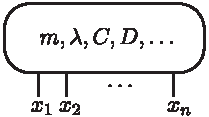
\includegraphics{pathintegral.pdf}}
	\end{split}
\end{equation}
where $\mathcal{T}$ denotes \emph{time ordering} (here the variables $x_1, x_2, \ldots$ denote \emph{spacetime locations}). Lagrangians are, in combination with the path integral, a wonderfully compact way specify QFTs in a way that makes locality, causality, and symmetries such as Lorentz invariance manifest. However, they have the not inconsiderable downside that it is often very hard to compute correlation functions except perturbatively around special points.  

We thus think of \emph{quantum theories}\footnote{The arguments of $n$-point correlation functions may be at unequal times and thus encode both kinematics and dynamics.}, being  in this case the specification of all $n$-point functions via the path integral above, as being parametrised by the (infinite) list of coupling constants $(m, \lambda, C, D, \ldots)$. We further imagine that the coupling constants are the coordinates for some fictitious infinite dimensional manifold $\mathcal{M}$ which we call the \emph{manifold of all theories}:
\begin{center}
	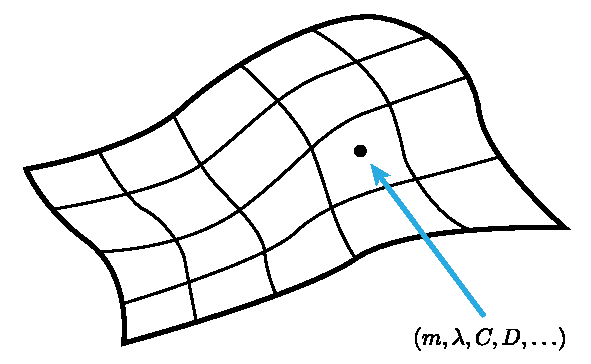
\includegraphics{manifold.pdf}
\end{center}
This ``manifold'' is rather poorly defined. 

It is important to steadfastly resist the temptation to give the coupling constants $(m, \lambda, C, D, \ldots)$ any operational interpretation whatsoever, despite the observation that, according to dimensional analysis, e.g., $m$ has units of mass. They are just parameters. (Recall that for us a quantity is deemed physical if there is an experiment that could, in principle, measure it.) 

To understand the manifold $\mathcal{M}$ we begin by first trying to understand the better behaved space $\mathcal{M}_{\Lambda}$ of \emph{regulated} or \emph{cutoff} quantum field theories with cutoff $\Lambda \ge 0$. What are these? Well, there are an infinite number of ways to define them, but one you can keep in mind is to simply put the theory on a lattice with lattice spacing $a = 1/\Lambda$. We emphasise, at this stage, that regulated theories are the only ones expected to make mathematical sense. You can think of a resident of $\mathcal{M}_{\Lambda}$  as some interacting theory of bosons and fermions hopping on a lattice with spacing $a=1/\Lambda$ with coupling constants $(m(\Lambda), \lambda(\Lambda), C(\Lambda), D(\Lambda), \ldots)$. (Here we explicitly indicate that the coupling constants are for a lattice theory with cutoff $\Lambda$.) This way of defining a cutoff QFT is certainly not the most elegant, but it does enjoy considerable advantages for evaluation on a computer. 

Once you have cut off a quantum field theory most, if not all, of the nasty divergences you've heard about disappear, and we only have to cope with more pedestrian divergences familiar to condensed matter physicists (e.g., the ``orthogonality catastrophe'' and ``infrared divergences''). 

We imagine that each of the spaces $\mathcal{M}_\Lambda$ are diffeomorphic via some map $f_\Lambda$ to a subspace of the (presumably better defined) common space $\mathcal{M}_{\text{reg}} \equiv \bigcup_{\Lambda \ge 0} \mathcal{M}_{\Lambda}$. One might be tempted to think that $\mathcal{M}_{\text{reg}}$ is already the space $\mathcal{M}$ of legitimate quantum field theories. However, this is really not the case: any theory in the space $\mathcal{M}_{\text{reg}}$ corresponds, by construction, to a lattice theory with a \emph{finite} cutoff $\Lambda$. This cutoff can be arbitrarily large but it must always be finite and thus there is always an underlying lattice structure (be it in momentum or position space or otherwise). A good analogy to the situation at hand is that of the rational numbers $\mathbb{Q}$ and the real numbers $\mathbb{R}$: any element of $\mathbb{Q}$ is expressible as $a/b$ with $a<\infty$ and $b < \infty$. However, something like $\sqrt{2}$ would need to be expressed as a rational number with infinitely large numerator and denominator, i.e., there are many numbers `missing' from $\mathbb{Q}$. 

The space $\mathcal{M}_{\text{reg}}$ is still missing some vital structure, namely, for any particular given theory in $\mathcal{M}_{\Lambda}$ parametrised by the coordinates $(m(\Lambda), \lambda(\Lambda), C(\Lambda), D(\Lambda), \ldots)$ we can always find a \emph{physically equivalent} theory $(m(\Lambda'), \lambda(\Lambda'), C(\Lambda'), D(\Lambda'), \ldots)$ in $\mathcal{M}_{\Lambda'}$ having a larger cutoff $\Lambda' > \Lambda$. What does this mean concretely? The standard answer is that the theory with coordinates $(m(\Lambda), \lambda(\Lambda), C(\Lambda), D(\Lambda), \ldots)$ is physically equivalent to $(m(\Lambda'), \lambda(\Lambda'), C(\Lambda'), D(\Lambda'), \ldots)$ if the \emph{low-order correlation functions of large-scale low-energy observables} as predicted by both theories are the same. This determines a map
\begin{equation}
	\mathcal{F}_{\Lambda,\Lambda'}: \mathcal{M}_\Lambda \rightarrow \mathcal{M}_{\Lambda'}
\end{equation}
In other words: if we make a prediction for low-energy large-scale observables using a theory with cutoff $\Lambda$ then a \emph{physically equivalent} theory in $\mathcal{M}_{\Lambda'}$ must give the same predictions for the original low-energy large scale observables. This map is not trivial to determine; this is where we need to do some physics! 

Suppose that the dependence of $\mathcal{F}_{\Lambda,\Lambda'}$ on $\Lambda$ and $\Lambda'$ is smooth.  Then we generate a \emph{flow} on $\mathcal{M}_{\text{reg}}$ 
\begin{equation}
	f_{\Lambda'}\circ \mathcal{F}_{\Lambda,\Lambda'}\circ f_\Lambda^{-1}   
\end{equation}   
according to the diagram
\begin{equation}
\xymatrix{
\mathcal{M}_{\Lambda} \ar[rr]^{\mathcal{F}_{\Lambda,\Lambda'}}
\ar[dr]_{f_\Lambda}\hole
&& \mathcal{M}_{\Lambda'} \ar[dl]^{f_{\Lambda'}}\\
& \mathcal{M}_{\text{reg}} }
\end{equation}
It is usually assumed  that that this flow on the infinite-dimensional space $\mathcal{M}_{\text{reg}}$ is generated by a \emph{vector field}, called the \emph{beta function}. A very special role is played by the \emph{fixed points} of this flow, as they correspond to genuine cutoff-free quantum field theories, i.e., theories of continuously many degrees of freedom. But does $\mathcal{M}_{\text{reg}}$ contain any such fixed points? This is an important question which leads us closer to a reasonable working definition of $\mathcal{M}$, namely as the original space $\mathcal{M}_{\text{reg}}$ with the ``missing'' points adjoined. (Again the analogy with $\mathbb{Q}$ is helpful here: fixed points of well-defined maps on $\mathbb{Q}$ can easily fail to be in $\mathbb{Q}$, for example, consider $f(x) = x^2-1$: the fixed points of this map are $x_{\pm} = \frac{1\pm\sqrt{5}}{2}$.) Thus we can tentatively think of $\mathcal{M}$ as the space of regulated theories with possibly missing fixed points of $\mathcal{F}_{\Lambda,\Lambda'}$ adjoined. It turns out that this picture is pretty close to the actual definition. Conformal field theories, being scale invariant, are then precisely fixed points.

\section{Quantum field theory and critical phenomena}
In this section we continue the description of the Wilsonian formulation of quantum field theory by describing how to exploit quantum field theory as an effective model of \emph{critical phenomena}. This, in turn, provides us with a general way to microscopically realise quantum fields. The treatment here owes much to Wilson and Kogut's original article \cite{wilson_renormalization_1974}. For the more rigourously minded, we enthusiastically recommend an article of Fr\"ohlich and Spencer \cite{frohlich_recent_1981}. In contrast to most treatises our treatment here is framed in the hamiltonian setting in order to make contact with the rest of our discussions.

Consider a very cold sample of some crystalline bulk matter. Imagine that at each crystal lattice site we have a quantum degree of freedom, e.g., a spin-$1/2$ degree of freedom. Suppose, further, there are competing interactions between the degrees of freedom, captured by a hamiltonian of the form
\begin{equation}\label{eq:latticemodel}
	H(q) = A + \sum_{j=1}^m q_j B_j,
\end{equation}
where, e.g., in the case $m=1$, $A$ and $B$ could be nearest-neighbour terms such as $A = \sum_{\langle j,k\rangle} \sigma^z_j\sigma_k^z$ and $B = \sum_{j} \sigma^x$, in which case we obtain the \emph{transverse Ising model}. (The discussion here is not at all limited to the transverse Ising model, and applies equally to all statistical mechanical systems.) Regulated quantum fields (with real-space regulator), particularly pure gauge fields, turn out to be precisely lattice models of this type. 

As long as $q$ is very large or very small the system is essentially in the ground state of either $A$ or $B$, which is usually one or more relatively boring product states. However, it can happen that as we vary $q$ from $0$ to $\infty$ that we encounter at a special value $q=q_c$ a \emph{quantum phase transition} \cite{sachdev_quantum_2011}. While we can't give a mathematical definition of what a quantum phase transition is, we'll know it when we see it; according to the standard yoga of critical phenomena as we approach $q=q_c$ quantum correlations build up in the system so that, e.g., the two-point function behaves something like
\begin{equation}\label{eq:correlator}
	\langle\Omega(q)| \sigma^\alpha_j\sigma^\beta_k|\Omega(q)\rangle \sim C_{\alpha\beta}e^{-\frac{|j-k|}{\xi(q)}},
\end{equation}
where $|\Omega(q)\rangle$ is the ground state of $H(q)$, $C_{\alpha\beta}$ are some constants, and $\xi(q)$ is the (dimensionless) \emph{correlation length}, measured in sites. Experience has shown us that the correlation length behaves as 
\begin{equation}
	\xi(q) \propto \frac{1}{|q-q_c|^\nu}.
\end{equation}
(The value of $\nu$ can depend on which side of $q_c$ the transition is approached and on the single-spin operators $\sigma^\alpha$ and $\sigma^\beta$.) If this is the first time you've encountered critical phenomena this may seem all rather unmotivated and arbitrary; but once you have seen this behaviour in 10, 20, 30, $\ldots$, different models you'll end up believing it quite happily.
Thus, as we approach the critical point, the system builds up ``clusters'' of correlations over larger and larger lengthscales which diverge at the critical point $q = q_c$. 

In an ideal world we'd just completely solve (\ref{eq:latticemodel}), and thus be able to calculate all the $n$-point correlation functions. Unfortunately we cannot do this except for some extremely special models, so we lower our expectations and focus on understanding just the \emph{large-scale behaviour} of $H(q)$, seeing as it is this behaviour which is easiest to access in an experiment anyway. One coarse way of extracting the long-range behaviour of $n$-point correlations functions such as (\ref{eq:correlator}) is to introduce the \emph{scaled correlations}
\begin{equation}
	G^{(\boldsymbol{\alpha})}_\vartheta(x_1, x_2, \ldots, x_n) \equiv  \left(\prod_{j=1}^n N_{\alpha_j}(\vartheta)\right) \langle\Omega(q(\vartheta))|\sigma^{\alpha_1}_{\vartheta x_1}\sigma^{\alpha_2}_{\vartheta x_2} \cdots \sigma^{\alpha_n}_{\vartheta x_n}|\Omega(q(\vartheta))\rangle,
\end{equation}
where $\vartheta$ is a \emph{scale parameter} which varies from $1$ to $\infty$, and $q(\vartheta)$ and $N_{\alpha}(\vartheta)$ are chosen so that $\lim_{\vartheta\rightarrow \infty} q(\vartheta) = q_c$ and the limit  
\begin{equation}
G^{(\boldsymbol{\alpha})}(x_1, x_2, \ldots, x_n) \equiv \lim_{\vartheta\rightarrow \infty}G^{(\boldsymbol{\alpha})}_\vartheta(x_1, x_2, \ldots, x_n)
\end{equation}
exists as $\vartheta\rightarrow\infty$. The positions $\vartheta x_j$ are required to lie on lattice sites along the limit: 
\begin{equation}
	\vartheta x_j \in \mathbb{Z}^d, \quad \text{so that} \quad x_j \in \frac{1}{\vartheta} \mathbb{Z}^d.
\end{equation}
The limiting scaled correlations $G^{(\boldsymbol{\alpha})}(x_1, x_2, \ldots, x_n)$, when they exist, are functions of \emph{continuous} spatial locations $x_1, x_2, \ldots, x_n\in \mathbb{R}^d$. Unfortunately the scaled correlation functions are still rather sensitive to certain UV lattice-scale fluctuations of the type arising in, e.g., Heisenberg antiferromagnetics where the single-spin expectation value flips its sign as one passes from even to odd lattice sites. (One of the technical contributions of this paper is to show how to ensure the existence of this limit by introducing a slightly modified definition with the added benefit of a better operational interpretation.) 

Because $G^{(\boldsymbol{\alpha})}(x_1, x_2, \ldots, x_n)$ are basically $n$-point functions of spin operators which are very far apart from each other much of the short-scale behaviour of the ground state $|\Omega(q)\rangle$ has been lost, leaving only a shadow in the long-distance scaling behaviour.

The final step in building an effective model for our critical lattice system in the scaling limit is to interpret the scaled correlation functions as the expectation values of some family of \emph{quantum fields} $\widehat{\phi}_{\alpha}(x)$ with respect to a quantum field state $|\Omega\rangle$. That is, for all tuples $(x_1, x_2, \ldots, x_n)$ and $(\alpha_1, \alpha_2, \ldots, \alpha_n)$ we interpret
\begin{equation}
	G^{(\boldsymbol{\alpha})}(x_1, x_2, \ldots, x_n) \equiv \langle\Omega|\widehat{\phi}_{\alpha_1}(x_1)\widehat{\phi}_{\alpha_2}(x_2)\cdots \widehat{\phi}_{\alpha_n}(x_n)|\Omega\rangle.
\end{equation}
Indeed, one can take the point of view that this is \emph{what a quantum field is}, namely, a collection of $n$-point functions for a lattice system approaching criticality. So far this discussion has focussed on kinematics; dynamics can be incorporated into this picture by studying the scaling limit of unequal-time correlation functions in a similar way.

We describe, in this paper, how to apply this Wilsonian view to different, indeed arbitrary, ways of parametrising QFTs. A key step is to first separating out states and observables into separate categories. As a crucial example, we'll show how to exploit \emph{tensor network states} to parametrise QFTs by implementing the continuum limit in the Wilsonian view directly on quantum states rather than lagrangians.

\section{Effective quantum field states}\label{sec:effectiveqftstates}

The core (and rather ambitious) objective of these notes is to come up with a definition of a \emph{quantum field state} which is hopefully applicable across a broad range of situations from systems with a lattice cutoff where it should match, e.g., the quantum field approximation to the transverse Ising model \cite{sachdev_quantum_2011}, to systems with a momentum cutoff, where it should match the results of standard perturbation theory, and, hopefully, beyond. However, the Wilsonian formulation described in the previous section, applying as it does to a hybrid of the observables and states, doesn't directly suggest a good definition; we'll need to employ a little imagination to extract a general formulation which looks a little friendlier for quantum information theorists. 

Casting an eye over the discussion in the previous section we isolate four core ingredients:
\begin{enumerate}
	\item A space of observables $\mathcal{A}_{\text{reg}}$ for \emph{regulated} theories which are mathematically well behaved. The space $\mathcal{A}_{\text{reg}}$ should be naturally parametrised by one or more a \emph{cutoffs}\footnote{It turns out that when you have more general cutoffs, e.g., by arbitrary nonregular spatial discretisations, then the additional structure you need is a \emph{partial order} on the space of cutoffs; this is usually canonical and we only discuss this problem in the context of two examples.} $\Lambda$, so that we can identify in $\mathcal{A}_{\text{reg}}$ the subspace $\mathcal{A}_{\Lambda}$ of theories with cutoff $\Lambda$. There is a great deal of arbitrariness here and we only pursue the details for two examples, namely, the momentum-space and real-space cutoffs.
	\item A state $\rho_0$ on the space of regulated observables. This specification allows us to restrict our attention to studying fluctuations around a given hypothesis for the vacuum of the effective theory. You should think of $\rho_0$ as being a representative of a given phase of matter. Technically it allows us to build a representation of our observables as operators on a Hilbert space.  
	\item A way to \emph{compare} the predictions of two theories with \emph{different} cutoffs -- an \emph{information metric}. We do this by agreeing on an operationally motivated distance measure on the \emph{state spaces} $\mathcal{S}_\Lambda$ of the $\mathcal{A}_\Lambda$s, and then extending this to the state space $\mathcal{S}_{\text{reg}}$ of \emph{all} regulated states on $\mathcal{A}_{\text{reg}}$.
	\item A definition for ``large-scale'' observables. This is done by specifying a \emph{completely positive map} $\mathcal{E}_\sigma : \mathcal{A}_{\text{reg}} \rightarrow \mathcal{A}_{\text{reg}}$, parametrised by one or more \emph{resolution} or \emph{scale parameters} $\sigma$, whose image is the convex set of all those effects measurable by large-scale observers (i.e., those measurement that we mere mortals can perform). It is only with respect to these observables that we actually compare two quantum field states.
\end{enumerate}  
As we argue below, once we've specified this ``minimal data'' we can exploit the Wilsonian view to define what is meant by a quantum field state. It is worth noting that it is possible, in some cases, to avoid specifying all four objects above and still end up with a meaningful notion of a quantum field state.

To concretely illustrate the components of the Wilsonian formulation we'll specifically refer to two important examples. The first example is a standard choice in QFT, namely that of the (hard or smooth) momentum cutoff. We briefly sketch the data required for the Wilsonian formulation in this case and connect it with the traditional description of perturbative interacting QFT by specifying a ``zooming-out'' CP map. The second example we consider, namely, the real-space cutoff requires a little more care to put it into a form appropriate for the Wilsonian formulation: here we encounter additional problems because we need to compare lattices with different lattice spacings. We show how Kadanoff blocking supplies us with a solution by supplying us with a ``zooming-out'' CP map describing the large-scale observables. 

\subsection{The momentum cutoff}
In this subsection we introduce the standard momentum cutoff and heuristically describe how it fits into the framework we sketched above. We focus on the simplest example, namely, a single scalar quantum field, although everything we write here applies immediately to fermion fields as well. Whether we can exploit a momentum cutoff to make sense of gauge fields and sigma models is far less clear; this is a topic for a more in-depth study.  

The first step in building our quantum field state is to construct a space $\mathcal{A}_{\text{reg}}$ of observables for a regulated theories parametrised by a cutoff $\Lambda$. We work in $(d+1)$ dimensions and parametrise our single-particle states in momentum space via the variable $k\in\mathbb{R}^d$; we are going to build a space of observables from the many particle space arising from (a subspace of) the complex Hilbert space $\mathfrak{h} \equiv L^2(\mathbb{R}^d)$. This construction is reasonably standard, and we content ourselves with a summary (see, e.g., \cite{bratteli_operator_1997} for further details). 

The \emph{canonical commutation relation} (CCR) algebra $\text{CCR}(\mathfrak{h})$ for $\mathfrak{h}$ is generated by \emph{annihilation} and \emph{creation} operators $a(f)$ and $a^\dag(f)$, with $f\in\mathfrak{h}$, which obey
\begin{equation}
	[a(f), a(g)] = 0 = [a^\dag(f), a^\dag(g)], \quad \text{and}\quad [a(f), a^\dag(g)] = (f,g)\mathbb{I},
\end{equation}
where $f, g\in \mathfrak{h}$ and $(\cdot, \cdot)$ is the inner product on $\mathfrak{h}$. Let $f\in \mathfrak{h}$: using $a(f)$ and $a^\dag(f)$ we build the \emph{smeared field operators}
\begin{equation}
	\widehat{\varphi}(f) \equiv \frac{1}{\sqrt2}(a(f) + a^\dag(f)), \quad \text{and} \quad \widehat{\pi}(f) \equiv \frac{-i}{\sqrt2}(a(f) - a^\dag(f)).
\end{equation}
Note that $\widehat{\varphi}(f)$ so defined is not quite the same as the field operator $\widehat{\phi}(f)$ familiar from textbook discussions of the scalar field: the difference is that $f$ is allowed to be \emph{complex} in our definition. We recover the standard field operators $\widehat{\phi}(f) = \widehat{\varphi}(f)$ and $\widehat{\pi}(f) = \widehat{\varphi}(if)$, when $f$ is real. These, in turn, may be used to build the \emph{Weyl}, or \emph{displacement}, operator
\begin{equation}
	W(f) \equiv e^{i\widehat{\varphi}(f)}.
\end{equation}
The Weyl operators satisfy, for $f, g \in \mathfrak{h}$, the identity
\begin{equation}
	W(f)W(g) = e^{-\frac{i}{2}\im(f,g)}W(f+g) = e^{-{i}\im(f,g)}W(g)W(f).
\end{equation}
We now focus on a special subspace $K$ of $\mathfrak{h}$, namely, that generated by single-particle functions $f$ with \emph{compact support}, i.e., functions which are zero outside a closed and bounded subset of momentum space $\mathbb{R}^d$. Using $K$ we build the subalgebra $\mathcal{A}_{\text{reg}}\subset \text{CCR}(\mathfrak{h})$ generated by the Weyl operators $W(f)$ with $f\in K$. This is, according to, e.g., Proposition 5.2.9 in \cite{bratteli_operator_1997}, a proper subalgebra of $\text{CCR}(\mathfrak{h})$. The regulated observables correspond to experimental apparatuses which are sensitive to momenta $k$ with magnitude smaller than some arbitrarily large (yet always finite) cutoff $|k| \le \Lambda$.

Now that we've defined a space of regulated observables we need to pick a state $\rho_0$ on $\mathcal{A}_{\text{reg}}$ from which to explore this phase of matter. There are many possibilities here, but the one most relevant for traditional quantum field theory is the ground state of the \emph{Klein-Gordon model}
\begin{equation}
	\widehat{H}_{\text{KG}} = \frac12\int d^3 {x}\, \left(\widehat{\pi}^2(\mathbf{x}) + (\nabla \widehat{\phi}(\mathbf{x}))^2 + m^2 \widehat{\phi}^2(\mathbf{x})\right).
\end{equation}
This model is written in terms of the field operators $\widehat{\phi}(\mathbf{x})$ and $\widehat{\pi}(\mathbf{x})$ which we haven't defined yet (such operators are not in $\mathcal{A}_{\text{reg}}$)! We are going to sidestep around this issue by just using $\widehat{H}_{\text{KG}}$ simply as a proxy for a state $\rho_0 \equiv |\Omega\rangle\langle \Omega|$ on $\mathcal{A}_{\text{reg}}$, and forget that we ever needed the as-yet poorly defined field operators at the point $\mathbf{x}$. The state we are going to build will be \emph{quasi-free}, or \emph{gaussian}, meaning that it is completely determined by its two-point functions or covariance matrix. Thus it sufficient to restrict our attention to the expectation values of the Weyl operators 
\begin{equation}\label{eq:charfun}
	\rho_0(W(f)) = \langle \Omega|W(f)|\Omega\rangle.
\end{equation}
A lengthy calculation shows (check!) that this is given by
\begin{equation}
	\rho_0(W(f)) = \exp\left(-\frac{1}{2}\int \frac{1}{\sqrt{|\mathbf{k}|^2 + m^2}}|\widehat{f}_r(\mathbf{k})|^2 + \sqrt{|\mathbf{k}|^2 + m^2}|\widehat{f}_i(\mathbf{k})|^2 \,\frac{d^3k}{(2\pi)^3} \right),
\end{equation}
where $\widehat{f}(\mathbf{k}) \equiv \int e^{i\mathbf{k}\cdot \mathbf{x}} f(\mathbf{x})\, d^3x$ and $\widehat{f} = \widehat{f}_r+ i \widehat{f}_i$. That the characteristic function (\ref{eq:charfun}) contains all the information we need is a consequence of the observation that we can differentiate the Weyl operators to obtain products of smeared field operators.

The next ingredient we need for the Wilsonian formulation is a distance measure between two states; we employ the \emph{Bures metric}
\begin{equation}
	D^2(\rho_1,\rho_2) \equiv 2\left(1-\tr\left(\sqrt{\sqrt{\rho_1}\rho_2\sqrt{\rho_1}}\right)\right).
\end{equation} 
for this purpose. This metric can be (somewhat tediously) evaluated \cite{marian_uhlmann_2012} between any two gaussian states. However, for the purposes of this discussion, it is sufficient to evaluate the distance between infinitesimally close states, whence
\begin{equation}
	D^2(\rho,\rho + \epsilon X) \approx \epsilon^2 \langle X, X\rangle_\rho,
\end{equation}
where $\langle X, Y\rangle_{\rho} \equiv \tr(X\Omega_\rho^{-1}(Y))$, with $\Omega_\rho(X) \equiv \frac12 (\rho X + X \rho)$.

The final ingredient we require for the Wilsonian formulation is a definition for the \emph{large-scale} observables available to experimentalists at lengthscale $\sigma > 0$. These are selected by a CP map $\mathcal{E}_\sigma$ modelling the combined effects of decoherence and the imprecisions of realistic detectors. This is a complex subject which certainly deserves a lengthy detailed treatment. Here we'll just content ourselves with a caricature of the actual CP map $\mathcal{E}_\sigma$ modelling these effects given by \emph{gaussian smearing}. This is the following gaussian CP map determined by its action 
\begin{equation}
	\mathcal{E}_\sigma(W(f)) \equiv e^{i\widehat{\varphi}(X(f))}e^{-\frac12(f,Yf)},
\end{equation}
on the Weyl operators, where
\begin{equation}
	X(f) \equiv g_\sigma\star f \equiv (g_\sigma \star f_r) + i (g_\sigma \star f_i),
\end{equation}
the $\star$ denotes convolution, $g_\sigma(x) = e^{-\frac{x^2}{\sigma}}/\sqrt{\pi\sigma}$, and $Y \equiv y \mathbb{I}$, $y> 0$. With this CP map in hand we henceforth define 
\begin{equation}
	\mathcal{A}_\sigma \equiv \mathcal{E}_\sigma (\mathcal{A}_{\text{reg}}).
\end{equation}

Let's now assemble the data required for the Wilsonian formulation for the momentum cutoff case here:
\begin{enumerate}
	\item The \emph{regulated observables} $\mathcal{A}_{\text{reg}}$ are given by the algebra $\text{CCR}(K)$ generated by functions $f$ with compact support.
	\item The reference state $\rho_0$ is determined by the characteristic function
	\begin{equation*}
		\rho_0(W(f)) = \exp\left(-\frac{1}{2}\int \frac{1}{\sqrt{|\mathbf{k}|^2 + m^2}}|\widehat{f}_r(\mathbf{k})|^2 + \sqrt{|\mathbf{k}|^2 + m^2}|\widehat{f}_i(\mathbf{k})|^2 \,\frac{d^3k}{(2\pi)^3} \right).
	\end{equation*}
	\item We employ the \emph{Bures metric} 
	\begin{equation*}
		D^2(\rho_1,\rho_2) \equiv 2\left(1-\tr\left(\sqrt{\sqrt{\rho_1}\rho_2\sqrt{\rho_1}}\right)\right)
	\end{equation*}
	as our distance measure.
	\item The \emph{large-scale observables at scale $\sigma$} are of the form
	\begin{equation*}
		M_\sigma \equiv \mathcal{E}_\sigma(M), \quad M\in \mathcal{A}_{\text{reg}}.	
	\end{equation*}
\end{enumerate}


\subsection{The real-space cutoff}
The real-space cutoff is implemented by putting the system on a lattice with (variable) lattice spacing $a$. In discussing the real-space cutoff case we encounter an additional problem which we did not (directly) have to engage with in the momentum cutoff case, namely, how do we compare two systems with different lattice spacing? 

We begin by building the space of observables for a one-dimensional system with a \emph{fixed} real-space cutoff, i.e., a lattice $L_a$ with spacing $a$: 
\begin{center}
	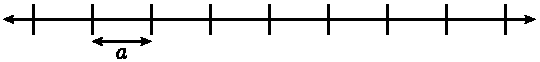
\includegraphics{lattice.pdf}
\end{center}
This is a regular partition of the real line $\mathbb{R}$ by a collection of lattice cells of the form $I_j \equiv [ja, (j+1)a)$, i.e., $L_a \equiv \{I_j\}_{j\in \mathbb{Z}}$. For concreteness we focus on the example a system where we associate a quantum spin-$1/2$ degree of freedom (i.e., a qubit) with each lattice \emph{cell}\footnote{We associate degrees of freedom with cells rather than vertices as we (usually) regard them as representing the averaged value of some physical quantity, e.g., angular momentum, over the cell.}, or \emph{link}, $I_j$. The Hilbert space for such a system would naively be the infinite tensor product of $\mathbb{C}^2$, one for each lattice cell. However, we avoid the discussion of how to make sense of this for the moment and instead describe the arguably more natural space of observables for this system. This space is built as follows: for any finite subset $\Lambda \subset L_a$ of lattice cells let $\mathcal{A}(\Lambda)$ be the tensor product of $M_2(\mathbb{C})$ over each $I_j\in \Lambda$. For $\Lambda_1\subset \Lambda_2$ we identify $\mathcal{A}(\Lambda_1)$ in a natural way with $\mathcal{A}(\Lambda_1)\otimes \mathbb{I}_{\Lambda_2\setminus \Lambda_1} \subset \mathcal{A}(\Lambda_2)$. For infinite $\Lambda \subset L_a$ denote by $\mathcal{A}(\Lambda)$ the $C^*$-closure of the increasing family of finite-dimensional algebras $\mathcal{A}(\Lambda_f)$ with $\Lambda_f \subset \Lambda$. What this means in words is that $\mathcal{A}(\Lambda)$ contains all observables which act on at most a finite number of spins as well as observables which are \emph{well approximated} by sequences of observables acting on at most a finite number of spins. The \emph{quasi-local algebra} is then $\mathcal{A}(L_a)$, and this is the space of observables we associate with our regulated system. 

To get a feel for what kinds of observables live in $\mathcal{A}(L_a)$ we consider a couple of examples. The simplest is a \emph{single-site operator}, e.g., $\sigma^z_j$ (we adopt the simpler subscript notation $A_j \equiv A_{I_j}$ for an operator acting nontrivially only on lattice cell $I_j$). An example of an observable well-approximated by a sequence of finite-support operators is $\sum_{j\ge 0} e^{-j}\sigma^z_0 \sigma_1^z  \cdots \sigma_{j-1}^z\sigma_j^z$. An important class of observables that \emph{do not} live in $\mathcal{A}(L_a)$ are the ``mean field''-type observables, e.g., $M_z \text{``$\equiv$''} \lim_{n\rightarrow\infty}\frac{1}{n}\sum_{j = 0}^{n-1} \sigma^z_j$ (here the scare quotes indicate that the limiting object doesn't make sense). Another type of observable that doesn't live in $\mathcal{A}(L_a)$ are given by the finite-rank projections $P$ and most spectral projections for bulk observables like $M_z$. This ``deficit'' of the observable set $\mathcal{A}(L_a)$ can be corrected by passing to a von Neumann algebra, however this requires the introduction of a reference state, a step we don't yet wish to take. 

The space $\mathcal{A}(L_a)$ is specifically tied to a lattice with a \emph{fixed} spacing $a$. However, the space $\mathcal{A}_{\text{reg}}$ of regulated observables should contain observables corresponding to experiments on systems with arbitrary (yet always nonzero) lattice spacing $a$. The way we accommodate this possibility is to build $\mathcal{A}_{\text{reg}}$ from the \emph{direct sum} of $\mathcal{A}(L_a)$ over a sequence of allowed values of the lattice spacing $a$. It is possible to allow any nonnegative value for $a$, but this is a little more awkward in practice. As we'll see, allowing $a$ to be an arbitrary simple dyadic rational of the form $2^{-j}$ will already suffice. The way to capture all these possible observables is then via the object 
\begin{equation*}
	\mathcal{A}_{\text{pre}} \equiv \bigoplus_{j \in \mathbb{Z}^+} \mathcal{A}(L_{2^{-j}}).
\end{equation*}
This is an economical way of allowing observables for lattices of arbitrarily small -- yet finite -- lattice spacing\footnote{The astute reader will notice that $\mathcal{A}_{\text{pre}}$ doesn't contain the identity. We'll mostly ignore this subtlety because an approximate identity suffices to yield a reasonable operational interpretation.}. The kind of physical situation modelled by the observable set $\mathcal{A}_{\text{pre}}$ is that of a system with a \emph{classical} dial controlling the lattice spacing (this can be implemented in the laboratory by, e.g., putting the sample in a liquid and increasing the pressure). A typical positive observable living in $\mathcal{A}_{\text{pre}}$ has the form of a finite convex combination $\sum_{l=1}^n M(a_l)$ of observables $M(a_l)\in\mathcal{A}(L_{a_l})$ for lattices with possibly different spacings $a_l\in\{1, \frac{1}{2}, \frac{1}{4}, \ldots\}$; such observables correspond to the experiment where a collection of coins are first flipped and, conditioned on the outcome, the observable $M(a_l)$ is subsequently measured. 

It turns out that the observable set $\mathcal{A}_{\text{pre}}$ doesn't quite correspond to the situation we wish to model -- it is a little too large. This is because there is no notion of whether an observable corresponds to the same physical quantity, only measured on a lattice with a different lattice spacing. The picture to have in mind here is that of a neutron scattering experiment where the same impinging beam scatters from the sample, regardless of the lattice spacing: 
\begin{center}
	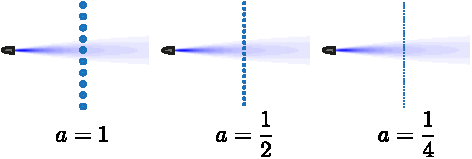
\includegraphics{decreasea.pdf}
\end{center}
To accommodate this additional structure we introduce an \emph{equivalence relation} on $\mathcal{A}_{\text{pre}}$ by introducing the subspace $N \subset \mathcal{A}_{\text{pre}}$ generated by all the differences $M_{a}-M_{a'}$, where $M_{a}$ and $M_{a'}$ are meant to correspond to the \emph{same} experiment, only with different lattice spacings $a$ and $a'$. Using $N$ we can finally define $\mathcal{A}_{\text{reg}}$:
\begin{equation}
	\mathcal{A}_{\text{reg}} \equiv \mathcal{A}_{\text{pre}}/N.
\end{equation}
The equivalence relation on observables, and subsequently, the definition of $N$, is determined by \emph{physics}, and no amount of abstract nonsense will assist us in going further. 

In order to prevent this discussion from becoming too ethereal we now consider a very particular concrete example in some detail. The physical picture we have in mind for this example is that of a quantum magnet modelled, e.g., by the ferromagnetic Heisenberg model in an external magnetic field:
\begin{equation}
	H = -\sum_{j\in\mathbb{Z}} \boldsymbol{\sigma}_j\cdot\boldsymbol{\sigma}_{j+1} + h\sigma^z_j,
\end{equation}
with ground state $|\Omega\rangle \equiv \bigotimes_{j\in\mathbb{Z}} |0\rangle$. The magnet is assumed to have some magnons, represented as $|1\rangle$ states at certain locations, propagating around. For a given lattice spacing the state $|1\rangle_{I_j}$ represents a quantum magnon in somewhere in $I_j$, i.e., completely delocalised across the lattice cell $I_j$. If we subdivide the lattice cell into two contiguous equal-sized pieces $I_j \equiv I_{2j}'\cup I_{2j+1}'$ then it ought to be the case that $|1\rangle_{I_j}$ is an equal superposition of the magnon being on the left and right sides:
\begin{equation}
	|1\rangle_{I_j} \equiv \frac{1}{\sqrt{2}} \left(|1\rangle_{I_{2j}'}|0\rangle_{I_{2j+1}'}+|0\rangle_{I_{2j}'}|1\rangle_{I_{2j+1}'}\right).
\end{equation}
So far this notion of equivalence has been described in terms of states rather than observables. To implement our equivalence relation in terms of observables we introduce the \emph{interpolation} unitary $U:\mathbb{C}^2\otimes \mathbb{C}^2\rightarrow \mathbb{C}^2\otimes \mathbb{C}^2$:
\begin{equation}
	U \equiv \begin{pmatrix} 1 & 0 & 0 & 0 \\ 0 & \frac{1}{\sqrt{2}} & -\frac{1}{\sqrt{2}} & 0 \\ 0 & \frac{1}{\sqrt{2}} & \frac{1}{\sqrt{2}} & 0 \\ 0 & 0 & 0 & 1\end{pmatrix}.
\end{equation}
Using $U$ we build the CP map (in the heisenberg picture):
\begin{equation}
	\mathcal{U}(A) \equiv U^\dag (A\otimes \mathbb{I}) U.
\end{equation}
This map identifies the observables for a given interval $I_j$ with the physically identical observables for two equal sized contiguous intervals $I_{2j}$ and $I_{2j+1}$. The corresponding CP map in the Schr\"odinger picture is given by
\begin{equation}
	\mathcal{U}^{*}(\rho) \equiv \tr_2( U \rho U^\dag),
\end{equation}
and has the property that it maps the state $|00\rangle$ to $|0\rangle$ and $\frac{1}{\sqrt{2}} \left(|10\rangle+|01\rangle\right)$ to $|1\rangle$. 

Using the map $\mathcal{U}$ we build the map 
\begin{equation}
	\mathcal{F}_{j,j+1} \equiv \bigotimes_{j\in 2\mathbb{Z}} \mathcal{U},
\end{equation}
which naturally acts from $\mathcal{A}_{2^{-j}}$ to $\mathcal{A}_{2^{-j+1}}$. The Schr\"odinger picture version $\mathcal{F}_j^{*}$ of $\mathcal{F}_{j}$ is nothing but a \emph{Kadanoff blocking} of the lattice where we block spins together in pairs, apply some blockwise unitary $U$, and then trace out every second spin:
\begin{center}
	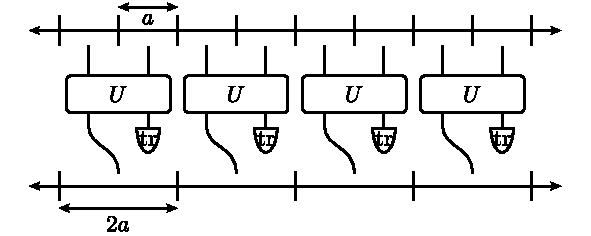
\includegraphics{kadanoff.pdf}
\end{center}
We then define, for all $j, k \in \mathbb{Z}^+$ with $j < k$, the map
\begin{equation}
	\mathcal{F}_{j,k}\equiv \mathcal{F}_{k-1,k}\circ \mathcal{F}_{k-2,k-1} \circ \cdots \circ \mathcal{F}_{j,j+1}
\end{equation}
representing a sequence of $k-j$ Kadanoff blocking operations.
Using $\mathcal{F}$ we finally introduce an equivalence relation $\sim$ by identifying $M \in \mathcal{A}_{2^{-j}}$ with $\mathcal{F}_{j,k}(M) \in \mathcal{A}_{2^{-k}}$. Thus we build the subspace $N\subset \mathcal{A}_{\text{pre}}$ generated by all differences $M_j - \mathcal{F}_{j,k}(M_j)$, for all $j<k$ and all $M_j\in \mathcal{A}_{2^{-j}}$, and hence define $\mathcal{A}_{\text{reg}} \equiv \mathcal{A}_{\text{pre}}/N$.
Thus we've arrived at the first ingredient required by the Wilsonian formulation, namely, a space $\mathcal{A}_{\text{reg}}$ of observables containing effects corresponds to experiments with respect to any allowed lattice with a finite yet non-zero spacing. 

We can now describe the space of $\mathcal{S}_{\text{reg}} \equiv \mathcal{S}(\mathcal{A}_{\text{reg}})$ of \emph{regulated field states}. The way to understand a state $\rho$ in this space is as an infinite direct sum $\rho_{\text{reg}} \equiv \bigoplus_{j\in \mathbb{Z}^{+}} \rho_{j}$ of states $\rho_{j} \in \mathcal{S}(\mathcal{A}_{2^{-j}})$, one for each lattice $L_{2^{-j}}$, such that for all $j<k$ the states $\rho_j$ and $\rho_k$ \emph{exactly} satisfy $\rho_j \equiv \mathcal{F}^{*}(\rho_k)$. In words: a regulated field state $\rho_{\text{reg}} \equiv \text{diag}(\rho_0, \rho_1, \rho_2, \ldots)$ is nothing but a sequence of states generated by Kadanoff blockings of each other. A simple example here is $\Omega \equiv (\rho_j)_{j\in \mathbb{Z}^+}$, where $\rho_j \equiv |\Omega_j\rangle\langle \Omega_j|$ with $|\Omega_j\rangle \equiv \bigotimes_{l\in \mathbb{Z}} |0\rangle$. However there are more complicated states inside $\mathcal{S}_{\text{reg}}$. For example, let $\chi_{[a,b)}:\mathbb{R}\rightarrow\mathbb{R}$ be the characteristic function
\begin{equation}
	\chi_{[a,b)}(x) = \begin{cases} 1,& \quad a\le x < b, \\ 0,& \quad \text{otherwise,}\end{cases}
\end{equation}
where $a,b\in\mathbb{R}$. Build the state
\begin{equation}
	|\chi_{[0,1)}\rangle_j \equiv 2^{-\frac{j}{2}}\sum_{k\in \mathbb{Z}} \chi_{[0,1)}(k2^{-j}) |k\rangle_j
\end{equation}
where 
\begin{equation}
	|k\rangle_j = \left(\bigotimes_{\substack{l\in\mathbb{Z} \\ l < k}} |0\rangle \right)\otimes |1\rangle \otimes\left(\bigotimes_{\substack{l\in\mathbb{Z} \\ l > k}} |0\rangle \right).
\end{equation}
One can verify that $|\chi_{[0,1)}\rangle_j\langle \chi_{[0,1)}| = \mathcal{F}_{j,k}^{*}(|\chi_{[0,1)}\rangle_k\langle \chi_{[0,1)}|)$ and thus we obtain a well-defined state, call it $\omega(\chi_{[a,b)})$, on $\mathcal{A}_{\text{reg}}$.

A plethora of interesting states may be built by exploiting the following \emph{right inverse} CP map $\mathcal{G}^{*}$ of $\mathcal{F}^{*}$, described in the Schr{\"o}dinger picture by
\begin{equation}
	\mathcal{G}_{j+1,j}^{*} \equiv \bigotimes_{j\in 2\mathbb{Z}} \mathcal{U}',
\end{equation}
where
\begin{equation}
	\mathcal{U}'(\rho) \equiv U(\rho\otimes |0\rangle\langle 0|) U^\dag.
\end{equation}
(There is no unique right inverse for $\mathcal{F}^{*}$. This is because replacing $|0\rangle$ by any other single qubit state in the definition of $\mathcal{U}'$ produces another inequivalent right inverse.)
One can confirm that
\begin{equation}
	\mathcal{F}_{j,j+1}^{*}\circ \mathcal{G}_{j+1,j}^{*} \equiv \mathcal{I}_j.
\end{equation}
We now see that the example presented above, namely $\omega(\chi_{[a,b)})$, can be constructed by applying $\mathcal{G}_{j+1,j}^{*}$ repeatedly to the initial state $|\chi_{[0,1)}\rangle_0$. Indeed, any state on $\mathcal{A}_{2^{-0}}$ can be exploited in the same way to produce a state on $\mathcal{A}_{\text{reg}}$.

This example is intended to be indicative of a much more general situation: let $L_a$ be a $D$-dimensional lattice of arbitrary quantum spins we replace the rather specific $\mathcal{F}$ channel built with an arbitrary Kadanoff blocking where $\mathcal{U}$ is now allowed to be an \emph{arbitrary} blockwise unitary. Then, just as above, we can construct $\mathcal{F}$, and hence another $\mathcal{A}_{\text{reg}}$.

The second ingredient required by the Wilsonian formulation is the specification of a ``hypothesis state'' 
$\rho_0$ on $\mathcal{A}_{\text{reg}}$. This state is also dictated by physics: it describes a restriction on the space of states we intend to model to those fluctuations around $\rho_0$. In condensed matter language the hypothesis state describes an initial starting point in some prespecified bulk phase of matter. The core idea of the Wilsonian formulation is that quantum fields are precisely given by the scaling limits of quantum phase transitions; thus quantum field states need to apply to systems approaching phase transitions: we use $\rho_0$ to build such states approaching by the addition of particles/fluctuations on $\rho_0$. It is too much to hope that we could describe regions of the phase diagram disconnected by phase transitions in terms of $\rho_0$: we would need to replace $\rho_0$ by another representative of a disconnected phase. A key example to have in mind here is that of a topologically trivial phase represented by, say, a product state $\rho_0$, and a topologically nontrivial phase represented by, say, a toric code \cite{kitaev_fault-tolerant_2003} ground state $\rho_0'$. There is a phase transition separating these two phases. We can model this transition from either side by a quantum field theory, but it is unreasonable to expect that fluctuations around $\rho_0$ will give us a good model for the topological phase $\rho_0'$ past the phase boundary. Technically speaking: $\rho_0$ and $\rho_0'$ belong to unitarily inequivalent representations of $\mathcal{A}_{\text{reg}}$. 

Once we've selected our representative hypothesis state $\rho_0$ we can obtain a Hilbert space modelling particles/fluctuations. We do this by exploiting the \emph{GNS representation}, which is another way of saying that we focus only on $\rho_0$ and states related to $\rho_0$ by the addition of at most a finite\footnote{Finite can mean $6.02\times 10^{23}$.} number of particles. The idea is now to think of the observables $A\in \mathcal{A}_{\text{reg}}$ themselves as kets $|A\rangle$ in some Hilbert space by introducing the (possibly degenerate or singular) inner product on $\mathcal{A}_{\text{reg}}$ via
\begin{equation}
	\langle A|B\rangle \equiv \rho_0 (A^\dag B).
\end{equation}
and write
\begin{equation}
	N_{0} \equiv \{A\in \mathcal{A}_{\text{reg}}\,|\, \rho_0(A^\dag A)=0\}
\end{equation}
for the regulated observables which are \emph{trivial} with respect to $\rho_0$. This is not entirely correct: we first need to identify any two observables $A$ and $A' = A + X$ differing by an observable $X\in N_0$. This is achieved by forming the quotient $\mathcal{H} \equiv \mathcal{A}_{\text{reg}}/N_0$; we now have that $\mathcal{H}$ is a legitimate Hilbert space. We think of a ket $|A\rangle$ as the state of the system where a ``particle'' of ``type'' $A$ has been added to the initial state $\rho_0$. The observables $A\in\mathcal{A}_{\text{reg}}$ can now be represented as operators $\pi(A)$ with matrix elements determined by
\begin{equation}
	\langle \phi|\pi(A)|\psi\rangle \equiv \rho_0(\phi^\dag A \psi),
\end{equation}
with $\phi,\psi \in  \mathcal{A}_{\text{reg}}/N_0$. 

The following little example illustrates this procedure. Suppose we have a qubit $\mathcal{A}\equiv M_2(\mathbb{C}^2)$ in the state $\rho_0 \equiv \left(\begin{smallmatrix}
p&0\\ 0&1-p
\end{smallmatrix}\right)$. A short calculation shows that $N_0$ is trivial, and that $\mathcal{H}$ is a four-dimensional space which we can construct by applying $A\otimes \mathbb{I}$ to the entangled state
\begin{equation}
	|\Omega\rangle \equiv \sqrt{p}|0\rangle|0\rangle + \sqrt{1-p}|1\rangle|1\rangle,
\end{equation}
to produce $|A\rangle \equiv A\otimes\mathbb{I}|\Omega\rangle$, so that  
\begin{equation}
	\langle A|B\rangle \equiv \langle\Omega|(A^\dag B) \otimes \mathbb{I}|\Omega\rangle = \tr(\rho_0 A^\dag B).
\end{equation}
Thus, the GNS representation is nothing other than the process of \emph{purification} in quantum information theory \cite{nielsen_quantum_2000}.

In our specific running example the GNS representation of $\mathcal{A}_{\text{reg}}$ afforded by the product state  $\Omega \equiv (\rho_j)_{j\in \mathbb{Z}^+}$, where $\rho_j \equiv |\Omega_j\rangle\langle \Omega_j|$ with $|\Omega_j\rangle \equiv \bigotimes_{l\in \mathbb{Z}} |0\rangle$, may be understood as follows. Firstly, the state $\mathcal{H}$ in the GNS Hilbert space  $|\Omega\rangle$ corresponding to $\rho_0$ is a product state at every scale, i.e., no matter on what lattice spacing you look it is a product state. This is our \emph{vacuum state}. Every other state $|\phi\rangle$ in $\mathcal{H}$ is obtained from $|\Omega\rangle$ by applying operators from $\mathcal{A}_{\text{reg}}$ to $|\Omega\rangle$; by construction $|\phi\rangle$ is equivalent to a superposition of product states at some lattice spacing $a_l = 2^{-l}$ which can only differ from $|0\rangle$ in a finite number of places, i.e.,  
\begin{equation}
	|\phi\rangle_l = \sum_{n=0}^\infty\sum_{j_1 < j_2 < \ldots< j_n \in \mathbb{Z}} \phi_{j_1,j_2, \ldots, j_n}|j_1,j_2, \ldots, j_n\rangle_l,
\end{equation} 
where $|j_1,j_2, \ldots, j_n\rangle_l$ is the infinite product state which is $|0\rangle$ except at locations $j_1$, $j_2$, $\ldots,$ $j_n$, where it is a $|1\rangle$ state. 
%Let's examine the equivalence class of states on $\mathcal{A}_{2^{-j}}$ determined by $|j_1,j_2, \ldots, j_n\rangle_l$: this can be specified using $\mathcal{G}^{*}$: we determine a state $\sigma(j_1,j_2, \ldots, j_n) \equiv (\sigma_k(j_1,j_2, \ldots, j_n))_{k=0}^\infty$ on $\mathcal{A}_{\text{reg}}$ from $|j_1,j_2, \ldots, j_n\rangle_l$ by setting 
%\begin{equation}
%	 \sigma_k(j_1,j_2, \ldots, j_n) = \begin{cases}
%	 	\mathcal{G}^{*}_{k,l}(|j_1,j_2, \ldots, j_n\rangle_l\langle j_1,j_2, \ldots, j_n|), &\quad k>l, \\
%	 	|j_1,j_2, \ldots, j_n\rangle_l\langle j_1,j_2, \ldots, j_n|, &\quad k = l, \\
%	 	\mathcal{F}^{*}_{l,k}(|j_1,j_2, \ldots, j_n\rangle_l\langle j_1,j_2, \ldots, j_n|), &\quad k<l. \\
%	 \end{cases}
%\end{equation} 
It turns out that we can canonically identify our Hilbert space $\mathcal{H}$ as a \emph{subspace} of \emph{Fock space} $\mathfrak{F}_+(L^2(\mathbb{R}, \mu))$ of bosons on the real line whose single-particle wavefunctions\footnote{Let $\mathcal{K}\subset L^2(\mathbb{R}, \mu)$ denote the vector subspace of $L^2(\mathbb{R}, \mu)$ of \emph{simple functions} spanned by linear combinations of all characteristic functions with dyadic rational endpoints. Any square-integrable function may be realised as a cauchy sequence of simple functions in $\mathcal{K}$, hence the closure of $\mathcal{K}$ is $L^2(\mathbb{R}, \mu)$.} are restricted to be characteristic functions of the form $\chi_{[a,b)}(x)$ where $a$ and $b$ are dyadic rational numbers, i.e., numbers of the form $\frac{m}{2^n}$, where $m\in \mathbb{Z}$ and $n\in \mathbb{Z}^{+}$. This representation is furnished by the identification
\begin{equation}
	 |j_1,j_2, \ldots, j_n\rangle_l \equiv a^\dag\left(\chi_{\left[\frac{j_1}{2^l}, \frac{j_1+1}{2^l}\right)}\right)a^\dag\left(\chi_{\left[\frac{j_2}{2^l}, \frac{j_2+1}{2^l}\right)}\right)\cdots a^\dag\left(\chi_{\left[\frac{j_n}{2^l}, \frac{j_n+1}{2^l}\right)}\right)|\Omega\rangle.
\end{equation} 
One can verify that indeed that the inner products between any two vectors in $\mathcal{H}$ and the corresponding pair of vectors in $\mathfrak{F}_+(L^2(\mathbb{R}, \mu))$ are identical so that this is indeed an isomorphism of Hilbert spaces. It turns out that the subspace of $\mathfrak{F}_+(L^2(\mathbb{R}, \mu))$ so constructed is actually equal to the whole of $\mathfrak{F}_+(L^2(\mathbb{R}, \mu))$: multiply occupied single-particles states such as 
\begin{equation}
	(a^\dag(\chi_{[a,b)}))^m |\Omega\rangle,
\end{equation}
appear to be missing from $\mathcal{H}$, however this is an illusion because we can arbitrarily well approximate any such multiply occupied state with states coming from residents of $\mathcal{H}$. Consider, for example,
\begin{equation}
	\begin{split}
		(a^\dag(\chi_{[0,1)}))^2 |\Omega\rangle &= \left(\frac{1}{\sqrt{2^m}}\sum_{j=0}^{2^m -1} a^\dag(\chi_{2^{-m}[j,j+1)}) \right)^2|\Omega\rangle \\
		&= \frac{1}{{2^m}}\sum_{j\not=k=0}^{2^m -1} a^\dag(\chi_{2^{-m}[j,j+1)})a^\dag(\chi_{2^{-m}[k,k+1)})|\Omega\rangle + |\delta_m\rangle \\
		&= \frac{1}{{2^m}}\sum_{j\not=k=0}^{2^m -1} a^\dag(\chi_{2^{-m}[j,j+1)})a^\dag(\chi_{2^{-m}[k,k+1)})|\Omega\rangle + O(2^{-m}) \\
		&\approx \frac{1}{{2^m}}\sum_{j\not=k=0}^{2^m -1} |j,k\rangle_m.
	\end{split}
\end{equation}
This approximation may be made arbitrarily good by taking $m\rightarrow \infty$. In this way we deduce that $\mathcal{H}$ is actually isomorphic to $\mathfrak{F}_+(L^2(\mathbb{R}, \mu))$. Thus the regulated continuum limit in this case is nothing but the space of bosons moving on the real line. 

Even though we've obtained that the kinematics $\mathcal{H}$ for the regulated observables are equivalent to bosons moving on the line we are still not done. Just as for the momentum-space cutoff case, we have that any state in $\mathcal{H}$ has an effective cutoff: any state in $\mathcal{H}$ is well-approximated by a converging sequence of states $|\phi\rangle_l$ at scale $l$. Thus for any state $|\phi\rangle$ there is a cutoff scale $2^l$ such that $|\phi\rangle$ is, for all practical observable purposes, equivalent to the cutoff state $|\phi\rangle_l$. Thus we come to our next ingredient, namely, the specification of a subset $\mathcal{A}_\sigma \subset \mathcal{A}_{\text{reg}}$ of observables corresponding to large-scale experiments at scale $\sigma$. 

The next vital ingredient for the Wilsonian formulation is the selection of an operationally motivated distance measure on $\mathcal{A}_{\text{reg}}$. We again employ the Bures metric on $\mathcal{S}(\mathcal{A}_{2^{-j}})$:
\begin{equation}
	D^2_j(\rho_1,\rho_2) \equiv 2\left(1-\tr\left(\sqrt{\sqrt{\rho_1}\rho_2\sqrt{\rho_1}}\right)\right).
\end{equation}
(Here we are assuming the states are representable as trace-class operators; we intend to be cavalier about such things throughout these notes. For the reader concerned about the lack of rigour at this point we simply mention that a sensible way to deal with this quantity is to go to the GNS representation afforded by the state $\rho_1$.)

It is a nontrivial question how this metric extends from $\mathcal{S}(\mathcal{A}_{2^{-j}})$ to $\mathcal{S}_{\text{reg}}$ in a natural way. We deal with this by defining, for any pair $\rho_1$ and $\rho_2$ of states in $\mathcal{S}_{\text{reg}}$ the metric
\begin{equation}
	D^2(\rho_1,\rho_2) \equiv \lim_{j\rightarrow\infty}  D^2_j(\rho_{1,j},\rho_{2,j}).
\end{equation}
The existence of this limit is guaranteed by the fact that $D^2_j(\rho_{1,j},\rho_{2,j})$ is a nonnegative bounded monotone increasing function of $j$, thanks to the fact that the Bures metric is \emph{monotone} and that $\rho_{1,j}$ (respectively, $\rho_{2,j}$) is the image of the CP map $\mathcal{F}_{j,k}^{*}$ applied to $\rho_{1,k}$ (respectively, $\rho_{2,k}$).



The final ingredient we need for a Wilsonian formulation is the identification of a subset $\mathcal{A}_\sigma$ of observables corresponding to an experiment at some large terrestrial scale $\sigma$. We achieve this by building a ``blurring'' CP map $\mathcal{E}_{\sigma}:\mathcal{A}_{\text{reg}}\rightarrow \mathcal{A}_{\text{reg}}$ and define 
\begin{equation}
	\mathcal{A}_\sigma \equiv \mathcal{E}_{\sigma}(\mathcal{A}_{\text{reg}}).
\end{equation}
There is a deal of arbitrariness here in how we define blurring maps; there is no abstract recipe we can appeal to. Instead we again need to do some physics. The following map may be argued to provide a reasonable model for observables accessible at scale $\sigma > 0$: we begin by introducing the Lindblad operator $\mathcal{L}^{(j)}:\mathcal{A}_{2^{-j}} \rightarrow \mathcal{A}_{2^{-j}}$, where
\begin{equation}
	\mathcal{L}^{(j)}(\cdot) = 2\sum_{k\in \mathbb{Z}} \left(\textsc{swap}_{k,k+1}(\cdot)\textsc{swap}_{k,k+1} - \mathcal{I}(\cdot)\right),
\end{equation}
and $\mathcal{I}$ is the identity superoperator. This Lindblad generator may then be exploited to define the CP map
\begin{equation}
	\mathcal{E}_\sigma^{(j)} \equiv e^{(\sigma 2^{j})^2\mathcal{L}^{(j)}}.
\end{equation} 
We set aside, for the moment, the question of the continuity of this operator: a relatively simple argument shows that it acts continuously on operators with finite support -- it is at least strongly continuous with respect to the strong-operator topology generated by the GNS representation afforded by the product state $|\Omega\rangle$). Physically speaking the CP map $\mathcal{E}_{\sigma}$ subjects operators to a diffusion process for a period of ``time'' $\tau = (\sigma 2^{j})^2$: for large times $\tau$ any local operator $A_k$ will evolve to an operator of the form $e^{\tau\mathcal{L}^{(j)}}(A_k) \approx \frac{1}{\sqrt{8\pi \tau}}\sum_l e^{-\frac{(l-k)^2}{8\tau}} A_l$.

Because this is a diffusion process we know that a typical operator will have wandered approximately $\sqrt{\tau} = \sigma 2^j$ sites from its initial position. Since the lattice spacing is $2^{-j}$ we see that an operator initially localised at some position will have wandered approximately a physical distance $\sigma$ from its initial position. The diffusion map $\mathcal{E}_\sigma^{(j)}$ can now be used to build a blurring map on $\mathcal{A}_{\text{reg}}$ in the following fashion. Firstly, note that the action of $\mathcal{E}_\sigma^{(j)}$ can be extended in a well-defined way to apply to all of $\mathcal{A}_{\text{reg}}$ exploiting the channels $\mathcal{F}$ and $\mathcal{G}$:
\begin{equation}
	\mathcal{E}_\sigma^{(j)}(A_k) = \begin{cases} \mathcal{E}_\sigma^{(j)}\circ\mathcal{F}_{k,j}(A_k), \quad k < j \\
	\mathcal{F}_{k,j}\circ\mathcal{E}_\sigma^{(j)}\circ\mathcal{G}_{k,j}(A_k), \quad k > j. \end{cases}
\end{equation}
Using the channel $\mathcal{E}_\sigma^{(j)}$ we arrive at our final definition
\begin{equation}
	\mathcal{E}_\sigma \equiv \lim_{j\rightarrow \infty} \mathcal{E}_\sigma^{(j)}.
\end{equation}
Here the limit must be taken with respect to a topology on $\mathcal{A}_{\text{reg}}$; we expect that the limit exists in the strong-operator topology, but it is plausible that it also exists for the norm topology (although, to be honest, we aren't that hopeful...) 

The limiting channel $\mathcal{E}_\sigma$ may be described in words as follows: suppose we have an observable $A_j$ on a lattice with spacing $2^{-j}$. First embed this operator into an equivalent fine-grained observable on the lattice with finer spacing $2^{-k}$ using the channel $\mathcal{F}_{j,k}$. Then subject this fine-grained observable to blurring according to $\mathcal{E}_\sigma^{(k)}$. As $k$ is taken larger and larger the result of this operation will be a sequence $\mathcal{E}_\sigma^{(k)}(A_j)$ of observables in $\mathcal{A}_{\text{reg}}$ on finer and finer lattices. These observables will be better and better approximated by a gaussian weighted mixture of translates of the initial operator. The actual action of this channel is depicted in the following figure. 

Finally, we define the large-scale observables at scale $\sigma$ to be the image of $\mathcal{A}_{\text{reg}}$ under $\mathcal{E}_\sigma$:
\begin{equation}
	\mathcal{A}_\sigma \equiv \mathcal{E}_\sigma(\mathcal{A}_{\text{reg}}).
\end{equation}

For the reader dissatisfied with the density of unproven assertions in previous the construction of the large-scale observables we supply here an alternative, presumably equivalent, construction.

\section{Quantum field states}\label{sec:qftcompletion}
In this section we finally present a definition for what a quantum field state actually is. Before we do this we'll present a motivating allegory for our definition. 

Suppose we can only measure distances using rulers with tick marks spaced at regular intervals given by fractions of some standard tick length $a_0$; the tick spacing $\epsilon a_0$ of a ruler is hence a positive rational ratio $\epsilon \in \mathbb{Q}^+$ of $a_0$. Owing to its canonical nature, we may as well set $a_0 = 1$ by convention. Thus all lengths \emph{measured} in terms of rational numbers. 

According to a ruler of accuracy $\epsilon$, two lengths $x$ and $y$ differing by less than $\epsilon$ are \emph{indistinguishable}, i.e., two points $x$ and $y$ are \emph{$\epsilon$ equivalent} if
\begin{equation}
	x\sim_\epsilon y \Leftrightarrow |x-y| < \epsilon. 
\end{equation} 
Even though all lengths are \emph{measured} in terms of rational numbers it turns out that there can be lengths which aren't expressible as a rational number, no matter how accurate the ruler, e.g., the length $x^\star = \sqrt{2}$. Obviously no one in possession of one of the allowed rulers could measure the length $x_{\epsilon} = n\epsilon$ to be anything other than a multiple $n$ of the ticklength $\epsilon$ found from $n = \lfloor x^\star/\epsilon \rfloor$. However, it is the case that after upgrading a ruler to another with ticklength $\epsilon'$ the newly measured length $x_{\epsilon'} \equiv n'\epsilon$, where $n' = \lfloor x^\star/\epsilon \rfloor$ can \emph{change}, because the ruler is more accurate. It is hence desirable to obtain some kind of \emph{specification} of a \emph{physical length} which encodes the results of all possible allowed measurements by rulers with arbitrarily good (but still finite!) ticklengths $\epsilon > 0$. The naive answer is just to use the specification provided by a \emph{sequence} of successively more accurate lengths:
\begin{equation}
	(x_n)_{n \in \mathbb{N}}, \quad x_n\in \mathbb{Q}^+.
\end{equation}
Now not all sequences can occur, only those which became more accurate as $n \rightarrow \infty$. That is, only those sequences $(x_\epsilon)_{n \in \mathbb{N}}$ enjoying the property that $\forall \epsilon, \exists N\in \mathbb{N}$ such that $\forall m,n\in \mathbb{N}$
\begin{equation}
	|x_n-x_m| < \epsilon,
\end{equation} 
are considered to correspond to a possible physical length. Rational lengths $x\in \mathbb{Q}^+$ have the representation $(x_n)_{n\in \mathbb{N}}$, with $x_n = x$, so this our definition of a physical length can accommodate the old one. The space of all these sequences is denoted $\widehat{\mathbb{R}}^+$. However, it is now possible that two apparently different sequences can correspond to the same length. This is solved by introducing the equivalence relation 
\begin{equation}
	(x_n)_{n \in \mathbb{N}} \sim (y_n)_{n \in \mathbb{N}} \Leftrightarrow \text{if $\forall \epsilon$, $\exists N\in \mathbb{N}$ such that $m,n>N$ we have $|x_n-y_n| < \epsilon$.} 
\end{equation}
Thus, the space of all possible physical lengths is defined to be $\mathbb{R}^+ \equiv \widehat{\mathbb{R}}^+/\sim$.

Of course this fairy tale is just an allegory for the construction of the real numbers by the process of \emph{completion} of the rational numbers, whereby ``continuous'' things (i.e., elements of $\mathbb{R}$) are constructed by sequences of ``not-so-continuous'' things (i.e., the positive ratioanl numbers)

Let's isolate some key features of this allegory. Firstly, we have the space of ``not-so-continuous'' \emph{regulated observables}, namely, our rulers with positive rational ticklength. Secondly, we have some kind of reference state relative to which all other states are defined: in our case this is just the length $a_0 = 1$. Thirdly, we have a way to talk about \emph{precision}, or \emph{closeness} allowing us to say when two objects are effectively \emph{indistinguishable}. Finally, we can talk about a subset of the observables corresponding to some scale. These are just the rulers with a ticklength larger than some constant. We then build the continuous objects as sequences of finite-accuracy objects modulo the equivalence relation that two such sequences represent the same object if they are indistinguishable for all accuracies.

Hopefully, with this foreshadowing, our definition of what a quantum field state is should not be too surprising. We hereby propose that a quantum field state is a \emph{sequence} of states $(\rho_n)_{n\in\mathbb{N}}$ of the regulated observables $\mathcal{A}_{\text{reg}}$ that look closer and closer to each other, as measured by observables in $\mathcal{A}_\sigma$, as $n$ grows. More precisely, fix some observable scale $\sigma$ and some precision $\epsilon$; then if there is some $N(\epsilon, \sigma) \in \mathbb{N}$ so that the expectation values of all the $A_\sigma\in \mathcal{A}_\sigma$ with respect to the states $\rho_n$ look closer and closer, i.e.,
\begin{equation}
	|\langle A_\sigma\rangle_m - \langle A_\sigma \rangle_n| \equiv |\tr(A_\sigma (\rho_m - \rho_n))| < \epsilon,
\end{equation}
for all $m,n>N(\epsilon,\sigma)$, then the observer will conclude the sequence is converging to \emph{some kind of limiting object} $\Omega$. This is a quantum field state. (For the more mathematically inclined: what we have done is set up a family of seminorms 
\begin{equation}
	D_{A_\sigma}(\rho, \sigma)
\end{equation}
on the Banach space dual $\mathcal{A}_{\text{reg}}^{\#}$ of $\mathcal{A}_{\text{reg}}$, and completed it with respect to the induced locally convex topology. There are some subtleties associated with this construction that need to be addressed, including, the question of whether $D_{A_\sigma}(\rho, \sigma)$ is a separating family.) The set of quantum field states is hence $\widehat{\mathcal{S}}_{\text{reg}}$, the set of Cauchy sequences of states in $\mathcal{S}_{\text{reg}}$. Just as for the rational numbers, any state $\rho$ on $\mathcal{A}_{\text{reg}}$ is automatically a quantum field state in this sense, simply by identifying it with the sequence $(\rho_n)_{n\in\mathbb{N}}$, with $\rho_n \equiv \rho$.

To add: discussion.


\section{Building Cauchy sequences: the renormalisation group}\label{sec:cauchyseqrg}

We've learnt that a quantum field state is nothing other than a \emph{Cauchy sequence} of regulated quantum field states. This is all well and good but we now need to argue that this definition includes states that physicists would recognise. This is the task we take up in this section; we argue that not only such sequences exist but also there are an embarrassment of riches of them. We then argue that this plenitude can cut down to a manageable level by imposing a simple hypothesis for their structure.

\subsection{The momentum cutoff}
Here we build a sequence of states on $\mathcal{A}_{\text{reg}}$ associated with interacting quantum field theories and argue they give rise to a Cauchy sequence. 

The first serious nontrivial quantum field theory is \emph{$\phi^4$ theory} with associated hamiltonian
\begin{equation}
	\widehat{H}_{\phi^4} = \int d^3 {x}\, \left(\frac12\widehat{\pi}^2(\mathbf{x}) + \frac12(\nabla \widehat{\phi}(\mathbf{x}))^2 + \frac12m^2 \widehat{\phi}^2(\mathbf{x}) + \frac{\lambda}{4!}\widehat{\phi}^4(\mathbf{x})\right).
\end{equation}
As written this operator suffers from some extremely serious problems. The worst is that, so far as we know, it actually isn't an operator! That is, if we apply it to states on which it should naively be well defined then we immediately encounter divergences. The simplest example is $|\Omega\rangle$, the ground state of the Klein-Gordon equation: the ``state'' $\int d^3 {x}\, \left(\frac{\lambda}{4!}\widehat{\phi}^4(\mathbf{x})\right) |\Omega\rangle$ is not even remotely normalisable. Thus we cannot even propose a candidate for the ground state of $\widehat{H}_{\phi^4}$ which might be a quantum field state. Given our definition of a quantum field state as a \emph{sequence} of regulated states we might go for the next best thing, namely, a sequence of ground states which morally ought to tend to the ground state of $\widehat{H}_{\phi^4}$ as the cutoff is removed. Thus we consider 
\begin{equation}
	\widehat{H}_{\phi^4}(\Lambda) = \int \frac{d^3 {k}}{(2\pi)^3}\, \left(\frac12\widehat{\pi}^2(\mathbf{k}) + \frac12(\mathbf{k}^2 + m^2)\widehat{\phi}^2(\mathbf{k}))  + \int \frac{d^3 {k}_1d^3 {k}_2d^3 {k}_3}{(2\pi)^3}\, \frac{\lambda}{4!}\widehat{\phi}^4(\mathbf{x})\right).
\end{equation}
where
\begin{equation}
	\widehat{\phi}(\mathbf{k}) = \int \frac{d^3 {k}}{(\sqrt{2\pi})^{3}} e^{-i\mathbf{k}\cdot \mathbf{x}} \widehat{\phi}(\mathbf{x})
\end{equation}


Recall that our large-scale observables at scale $\sigma$ are determined in the Heisenberg picture by a CP map $\mathcal{E}_\sigma$ which acts by embedding or ``spreading out'' the observables across the UV degrees of freedom. In the Schr\"odinger picture this CP acts dually as $\mathcal{E}_\sigma^*$ where it is a \emph{coarse graining} map that essentially acts as a partial trace. Indeed, in the case of the hard momentum cutoff it is precisely a partial trace over the large momentum degrees of freedom.  Now, suppose we have some reduced density operator $\rho_\sigma$ from which we'd like to build a Cauchy sequence, i.e., from which we'd like to remove the UV regulator. To do this we need to ``put back in'' the state on the degrees of freedom between $\sigma$ and a UV cutoff $\Lambda$ in a way that would be consistent for all $\sigma < \Lambda$. This is the same as looking for a sequence $(\rho_{\Lambda_n})_{n=1}^\infty$ of states with the property that
\begin{equation}
\rho_{\Lambda_m} = \tr_{(\Lambda_m,\Lambda_n]}(\rho_{\Lambda_n}), \quad \Lambda_m < \Lambda_n.
\end{equation}
I.e., the state $\rho_{\Lambda_n}$ must be an \emph{extension} or, improperly, a \emph{purification}, of $\rho_{\Lambda_m}$ onto the larger bipartite system comprising the original interval $\Lambda_m$ and the complement of $\Lambda_m$ in $\Lambda_n$. Now there are an infinite number of extensions/purifications for any given state, so there are an infinite number of possible sequences. These are all Cauchy. In fact, even better, they are \emph{exactly} convergent sequences! 
What is happening here is that we are finding the \emph{inverse} of a many to one map (the coarse graining map $\mathcal{E}_\sigma$). Because the map is many to one there are, by definition, many inverses, each of which has every right to be called a UV completion or continuum limit. What an embarrassment of riches! 

We have every right to be dissatisfied and suspicious with the proposed solution above. As the astute reader will no doubt observe: the sequences $(\rho_{\Lambda_n})_{n=1}^\infty$ are not useful for physics because how could we ever decide which one is the correct one by doing experiments? Well, you know what, tough luck: to quote Polchinski, ``nobody ever promised you a rose garden''. This is just the way things are: it is simply the case that something bizarre and crazy could turn up at any moment in our particle accelerators as we upgrade them to access more an more observables. There is no mathematical proof that could ever exclude this possibility apart from our desire for the universe to be kind to us and be explainable. You just have to learn to live with this. 

The way we implement the constraint of ``explainability'' is to demand that our states are, at least in principle, \emph{parametrisable} in terms of a finite number of numbers, or \emph{coupling constants}. Traditionally this is carried 


To add: Wilson's triangle of renormalisation.

\begin{center}
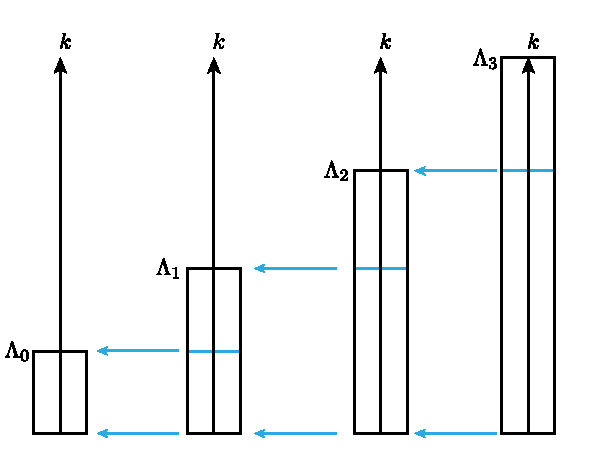
\includegraphics{rginverse.pdf}
\end{center}



We then define a \emph{field state} to be a sequence\footnote{More generally we'll need to specify field states by \emph{nets} $\phi_\Lambda \in \mathcal{F}$, $\Lambda\in\mathbb{R}^+$.} $\phi_n\in\mathbb{F}$, $n\in\mathbb{N}$, of field states such that for all values of the resolution parameters $r$, $\exists N\in \mathbb{N}$ such that $\forall m,n > N$ the states $\phi_m$ and $\phi_n$ are effectively indistinguishable at resolution $r$. Thus we have come to the idea of a \emph{Cauchy sequence} of regularised field states. The process of finding a Cauchy sequence, i.e., of building a sequence such that $\phi_n$ is Cauchy, is known as the \emph{renormalisation group}.


To add: finite-size scaling plots.


\section{Discussion}\label{sec:discussion}




\bibliography{What-is-a-quantum-field-state}

%\appendix


\end{document}  


